\chapter{\bfseries Mô Hình Kane Mở Rộng và Lý Thuyết Nhiễu Loạn $\mathbf{L\ddot{o}wdin}$}
\label{Chapter3} % For referencing the chapter elsewhere, use \ref{Chapter1} 
Cho tới lúc này chúng ta đã tính được gần đúng cấu trúc vùng năng lượng của chất bán dẫn, nhưng để có độ chính xác cao  ta sẽ kết hợp phương pháp kp với gần đúng là 14-band , ta sẽ tính lại tương tự như phần 4 dãy, nhưng ta sẽ thây đổi các Hamiltonian ở vùng hóa trị bằng các ma trận tính được nhờ phương pháp L$\ddot{o}wdin$ 
ta viết lại phương trình Schr$\ddot{o}$dinger như sau:
\begin{equation}
\left(\frac{\mathbf{p}^2}{2m_0} +\mathbf{V}_0\left(\mathbf{r}\right) + \mathcal{H}_{SO}\right)\psi_{m\mathbf{k}}\left(\mathbf{r}\right) = E_{m\mathbf{k}}\psi_{m\mathbf{k}}\left(\mathbf{r}\right)
\end{equation}
các đại lượng này ta đã định nghĩa ở các mục trước và ta cũng biến đổi tương tự ta có phương trình sau:
\begin{equation}
\sum_{n'}\mathcal{H}_{nn'}\left(\mathbf{k}\right) a_{m\mathbf{k}}^{n'} = E_{m\mathbf{k}}a_{m\mathbf{k}}^n
\end{equation} 
 ở đây 
\begin{equation}
\mathcal{H}_{nn'}\left(\mathbf{k}\right) = \left(E_0^n +\frac{\hbar^2 k^2}{2m_0}\right)\delta_{nn'} + \frac{\hbar}{m_0}\mathbf{k.p_{nn'}} + \Delta_{nn'}
\end{equation} 
số hạng thứ nhất trong phương Hamiltonian trình trên mô tả thành phần ma trận chéo hóa của điện tử tự do, còn $\Delta_{nn'}=\langle u_n|\mathcal{H}_{SO}|u_{n'}\rangle$ miêu tả số hạng ma trận không chéo hóa của spin-orbit và số hạng không chéo hóa ma trận mômen động lượng.
\begin{equation}
\mathbf{p_{nn'}}=\Bigl\langle u_n\Bigl\vert \mathbf{p}+\frac{\hbar}{4m_0c^2}\left(\boldsymbol{\sigma}\times\boldsymbol{\nabla V_o}\right)\Bigr \vert u_{n'}\Bigr\rangle
\end{equation}\\
Trong bức tranh tight-binding, mô hình Kane mở rộng sử dụng 14 band trong đó gồm có các thành phần bonding ứng với vùng $\Gamma_{8v},\Gamma_{7v}$ thuộc phân lớp p của vùng hóa trị, được mô tả bởi các hàm sóng ở dưới thông qua các trạng thái (X,Y,Z) và vùng dẫn tương ứng với các  antibonding s* và antibonding p* được mô tả thông qua các trạng thái (S),($X^{'},Y^{'},Z^{'}$) của vùng $\Gamma_{6c},\Gamma_{8c},\Gamma_{7c}$.

Nếu ta xét các hình thức trên thông qua toán học tức là lý thuyết nhóm  thì trạng thái s tương ứng mômen động lương quỹ đạo $l=0$ được trình bày bởi một biểu diễn $\mathcal{D}_0^{-}$ của một nhóm $\mathcal{R}=SU(2)\times C_i$ với một phép quay đầy đủ, và ta biến đổi nó thông qua phép biểu diển bất khả quy $\Gamma_1$ của nhóm điểm $T_d$ (vùng dẫn $\Gamma_1^{c}$) còn trạng thái p ứng với $l=1$ biến đổi thành $\Gamma_5$ (vùng dẫn $\Gamma_5^{c},$ vùng hóa trị $\Gamma_5^{v}$), chúng ta cũng cần chú ý rằng trong cấu trúc tinh thể kim cương b-bonding ở vùng hóa trị là chẳn ($\mathcal{D}_1^{+}$ thuộc $\mathcal{R}$,$\Gamma_5^{+}$ thuộc $\mathcal{O}_h$) còn b-antibonding ở vùng dẫn là lẻ ($\mathcal{D}_1^{-}$ thuộc $\mathcal{R}$,$\Gamma_5^{-}$ thuộc $\mathcal{O}_h$). Sự phân loại tính đối xứng của vùng năng lượng trong mô hình Kane mở rộng được tóm tắt trong bản 4.2.\\
Theo Koster [21] các mối liên hệ giửa hai phép biểu diễn bất khả quy $T_d$ và $\mathcal{O}_h$ có dạng sau:
\begin{table}[ht]
\caption{Mối liên hệ giửa $T_d$ vs $\mathcal{O}_h$}
% title of Table
\centering
% used for centering table
\begin{tabular}{c c c}
% centered columns (4 columns)
\hline\hline %inserts double horizontal lines
$\mathcal{O}_h$ &$\longrightarrow$&$ T_d$\\[0.5ex]
% inserts table
%heading
\hline
$\Gamma_1^{+}$ &$\longrightarrow$ &$\Gamma_1$\\
$\Gamma_2^{-}$ &$\longrightarrow$ &$\Gamma_1$\\
$\Gamma_4^{-}$ &$\longrightarrow$ &$\Gamma_5$\\
$\Gamma_5^{+}$ &$\longrightarrow$ &$\Gamma_5$\\
$\Gamma_6^{-}$ &$\longrightarrow$ &$\Gamma_7$\\
$\Gamma_7^{+}$ &$\longrightarrow$ &$\Gamma_6$\\[1ex]
\hline
\end{tabular}
\label{table:nonlin}
\end{table}
\begin{table}[hc]
\caption{Sự phân loại tính đối xứng của vùng năng lượng trong Kane $T_d$ vs $\mathcal{O}_h$ Ref[22]}
\centering
\begin{tabular}{c}
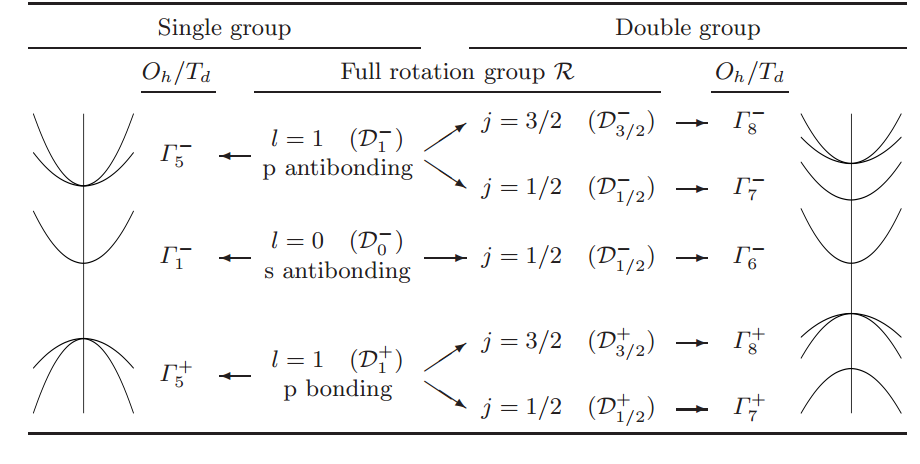
\includegraphics[width=1.0\textwidth, height=230px]{./Figures/hinh3.png}
\end{tabular}
\label{table:Symmetry}
\end{table}
\section{Mô hình Kane Mở rộng}
Khi thực hành trong tính toán ta bỏ đi số hạng thứ 2 trong phương trình trên (4.1) xem [23,20], trong mô hình $14\times14$ ta chọn 6 bonding vùng hóa trị(p) và 2 antibonding lớp ($s^*$), 6 antibonding lớp($p^*$) vùng dẫn tương tự ta chọn hàm sóng cơ sở trong hệ tọa độ hình cầu [23,9] $\vert jm\rangle $ theo trục lượng tử hóa [001]:\\
\emph{Đối với vùng} $\Gamma_{8c}$:
\[
u_1 = \left | \frac{3}{2},+\frac{3}{2}\right\rangle_{c^{'}}=\frac{-1}{\sqrt{2}}\left(
\begin{array}{cc}
X^{'} + iY^{'}\\
0
\end{array}
\right)
\qquad
u_2 = \left | \frac{3}{2},+\frac{1}{2}\right\rangle_{c^{'}}=\frac{-1}{\sqrt{6}}\left(
\begin{array}{cc}
-2Z^{'}\\
X^{'} + iY^{'}
\end{array}
\right)
\]
\[
u_3 = \left | \frac{3}{2},-\frac{1}{2}\right\rangle_{c^{'}}=\frac{1}{\sqrt{6}}\left(
\begin{array}{cc}
X^{'} - iY^{'}\\
2Z^{'}
\end{array}
\right)
\qquad
u_4 = \left | \frac{3}{2},-\frac{3}{2}\right\rangle_{c^{'}}=\frac{1}{\sqrt{2}}\left(
\begin{array}{cc}
0 \\
X^{'} - iY^{'}
\end{array}
\right)
\]
\emph{Đối với vùng} $\Gamma_{7c}$:
\[
u_5 = \left | \frac{1}{2},+\frac{1}{2}\right\rangle_{c^{'}}=\frac{-1}{\sqrt{3}}\left(
\begin{array}{cc}
Z^{'}\\
X^{'} + iY^{'}
\end{array}
\right)
\qquad
u_6= \left | \frac{1}{2},+\frac{-1}{2}\right\rangle_{c^{'}}=\frac{-1}{\sqrt{3}}\left(
\begin{array}{cc}
X^{'} - iY^{'}\\
-Z^{'}
\end{array}
\right)
\]
\emph{Đối vói vùng} $\Gamma_{6c}$:
\[
u_7 = \left | \frac{1}{2},+\frac{1}{2}\right\rangle_{c}=\left(
\begin{array}{cc}
S\\
0\end{array}
\right)
\qquad
u_8= \left | \frac{1}{2},+\frac{-1}{2}\right\rangle_{c}=\left(
\begin{array}{cc}
0\\
S
\end{array}
\right)
\]
\emph{Đối với vùng} $\Gamma_{8v}$:
\[
u_9 = \left | \frac{3}{2},+\frac{3}{2}\right\rangle_{v}=\frac{-1}{\sqrt{2}}\left(
\begin{array}{cc}
X + iY\\
0
\end{array}
\right)
\qquad
u_{10}= \left | \frac{3}{2},+\frac{1}{2}\right\rangle_{v}=\frac{-1}{\sqrt{6}}\left(
\begin{array}{cc}
-2Z\\
X + iY
\end{array}
\right)
\]
\[
u_{11} = \left | \frac{3}{2},-\frac{1}{2}\right\rangle_{v}=\frac{1}{\sqrt{6}}\left(
\begin{array}{cc}
X - iY\\
2Z
\end{array}
\right)
\qquad
u_{12} = \left | \frac{3}{2},-\frac{3}{2}\right\rangle_{v}=\frac{1}{\sqrt{2}}\left(
\begin{array}{cc}
0 \\
X - iY
\end{array}
\right)
\]
\emph{ Đối vói vùng} $\Gamma_{7v}$:
\[
u_{13} = \left | \frac{1}{2},+\frac{1}{2}\right\rangle_{v}=\frac{-1}{\sqrt{3}}\left(
\begin{array}{cc}
Z\\
X^ + iY
\end{array}
\right)
\qquad
u_{14}= \left | \frac{1}{2},+\frac{-1}{2}\right\rangle_{v}=\frac{-1}{\sqrt{3}}\left(
\begin{array}{cc}
X - iY\\
-Z
\end{array}
\right)
\]
và ta định nghĩa các ma trận mômentum và tương tác spin-orbit bởi các thông số sau [24,20,22]
\begin{align}
&\frac{\hbar}{m_0}\langle S|p_x|X\rangle = \frac{\hbar}{m_0}\langle S|p|_y|Y\rangle = \frac{\hbar}{m_0}\langle S|p_z|Z\rangle = P \notag \\
&\frac{\hbar}{m_0}\langle S|p_x|X^{'}\rangle = \frac{\hbar}{m_0}\langle S|p_y|Y^{'}\rangle = \frac{\hbar}{m_0}\langle S|p_z|Z^{'}\rangle = iP^{'} \notag\\
&\frac{\hbar}{m_0}\langle X|p_x|Z^{'}\rangle = \frac{\hbar}{m_0}\langle Y|p_y|X^{'}\rangle = \frac{\hbar}{m_0}\langle Z|p_x|Y^{'}\rangle = Q \notag\\
&\frac{-3i\hbar}{4m_0} \langle X|\left(\boldsymbol{\nabla}V_0\times p \right)_{y}|Z\rangle = \frac{-3i\hbar}{4m_0^2c^2}\langle Y|\left(\boldsymbol{\nabla}V_0\times p\right)_z|X\rangle = \frac{-3i\hbar}{4m_0^2c^2}\langle Z|\left(\boldsymbol{\nabla}V_0\times p\right)_x|Y\rangle =\Delta_0 \notag\\
&\frac{-3i\hbar}{4m_0} \langle X^{'}|\left(\boldsymbol{\nabla}V_0\times p \right)_{y}|Z^{'}\rangle = \frac{-3i\hbar}{4m_0^2c^2}\langle Y^{'}|\left(\boldsymbol{\nabla}V_0\times p\right)_z|X^{'}\rangle = \frac{-3i\hbar}{4m_0^2c^2}\langle Z^{'}|\left(\boldsymbol{\nabla}V_0\times p\right)_x|Y^{'}\rangle =\Delta_0^{'} \notag\\
&\frac{-3i\hbar}{4m_0} \langle X|\left(\boldsymbol{\nabla}V_0\times p \right)_{y}|Z^{'}\rangle = \frac{-3i\hbar}{4m_0^2c^2}\langle Y|\left(\boldsymbol{\nabla}V_0\times p\right)_z|X^{'}\rangle = \frac{-3i\hbar}{4m_0^2c^2}\langle Z|\left(\boldsymbol{\nabla}V_0\times p\right)_x|Y^{'}\rangle =i\Delta_0^{-} \notag \\
-&\frac{1}{2\sqrt{3}}\frac{\hbar^2}{m_0^2c^2}\langle X|\frac{\partial V_0}{\partial y}|Z\rangle = -\frac{1}{2\sqrt{3}}\frac{\hbar^2}{m_0^2c^2}\langle Y|\frac{\partial V_0}{\partial z}|X\rangle = -\frac{1}{2\sqrt{3}}\frac{\hbar^2}{m_0^2c^2}\langle Z|\frac{\partial V_0}{\partial x}|Y\rangle = C_k
\end{align}

\begin{figure}[hc]
\centering
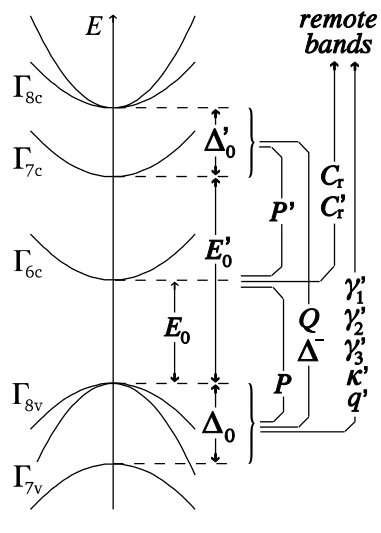
\includegraphics[width=0.50\textwidth]{./Figures/band.png}
%\rule{35em}{0.5pt}
\caption[Giản đồ cấu trúc vùng năng lượng 14 band mô hình Kane]{Giản đồ cấu trúc vùng năng lượng 14 band mô hình Kane với các tham số $P,P^{'},Q,\Delta_0,\Delta_0^{-},C_k $ được định nghĩa ở trên Ref[22].}
\end{figure}


\section{Phân tích các thành phần Hamiltonian}
\begin{enumerate}
\item[1/]\textbf{Số hạng tương tác kp:} $\langle u_i|\mathcal{H}_{kp}|u_j\rangle$
ký hiệu các trạng spin up$| \uparrow\rangle$, và spin down$|\downarrow\rangle$ và có tính chất sau:
\begin{align}
\langle \uparrow |\uparrow\rangle = \langle\downarrow |\downarrow\rangle =1,\langle \uparrow |\downarrow\rangle = \langle\downarrow |\uparrow\rangle =0
\end{align}
\begin{align*}
\mathcal{H}_{17}&=\frac{\hbar}{m_0}\Bigl\langle u_1\Bigl\vert \mathbf{kp}\Bigr\vert u_7\Bigr\rangle = \frac{-\hbar}{\sqrt{2}m_0}\Bigl\langle X^{'} -iY^{'}\Bigr\vert\mathbf{kp}\Bigl\vert S\Bigr\rangle \Bigl\langle\Bigl\uparrow \Bigl\vert \Bigr\uparrow\Bigr\rangle 
= \frac{-\hbar}{\sqrt{2}m_0}\Bigl[\Bigl\langle X^{'}\Bigl\vert \mathbf{kp}\Bigr\vert S\Bigr\rangle -i\Bigl\langle Y^{'}\Bigl\vert \mathbf{kp}\Bigr\vert S\Bigr\rangle\Bigr] \\
&=\frac{-\hbar}{\sqrt{2}m_0}\Bigl[\Bigl\langle X^{'}\Bigl\vert \mathbf{k_x p_x}\Bigr\vert S\Bigr\rangle -i\Bigl\langle Y^{'}\Bigl\vert \mathbf{k_x p_x}\Bigr\vert S\Bigr\rangle\Bigr]=\frac{1}{2}iP^{'}\left(k_x -ik_y\right)=\frac{1}{\sqrt{2}}iP^{'}k_{\_}
\end{align*}
\begin{align*}
\mathcal{H}_{71}&=\frac{\hbar}{m_0}\Bigl\langle u_7\Bigl\vert \mathbf{kp}\Bigr\vert u_1\Bigr\rangle  =
\frac{-\hbar}{\sqrt{2}m_0}\Bigl\langle S\Bigl\vert\mathbf{kp}\Bigr\vert X^{'} +iY^{'}\Bigr\rangle \Bigl\langle \Bigl\uparrow \Bigl\vert  \Bigr\uparrow
\Bigr\rangle =
\frac{-\hbar}{\sqrt{2}m_0}\Bigl[\Bigl\langle S\Bigl\vert \mathbf{kp}\Bigl\vert X^{'}\Bigr\rangle + i\Bigl\langle S\Bigl\vert \mathbf{kp}\Bigr\vert Y^{'}\Bigr\rangle\Bigr]\\
&=\frac{-\hbar}{\sqrt{2}m_0}\Bigl[\Bigl\langle S\Bigl\vert \mathbf{k_x p_x}\Bigr\vert X^{'}\Bigr \rangle +i\Bigl\langle S\Bigl\vert \mathbf{k_x p_x}\Bigr\vert Y^{'} \Bigr\rangle\Bigr]
=\frac{-1}{2}iP^{'}\left(k_x +ik_y\right)=\frac{-1}{\sqrt{2}}iP^{'}k_{+}
\end{align*}
để ý $\mathcal{H}_{71} = \left(\mathcal{H}_{17}\right)^*$, các số hạng kp còn lại ta tính tương tự.
\item[2/]\textbf{Số hạng tương tác SO}:\\
ta chú ý $\sigma_x|\uparrow\rangle = |\downarrow\rangle,\sigma_x|\downarrow\rangle = |\uparrow\rangle,\sigma_y|\uparrow\rangle = -i|\uparrow\rangle,\sigma_y|\downarrow\rangle = i|\downarrow\rangle,\sigma_z|\uparrow\rangle = |\uparrow\rangle,\sigma_z|\downarrow \rangle = |\downarrow\rangle$
\begin{align*}
\mathcal{H}_{11}&=\Bigl\langle u_1\Bigl\vert \boldsymbol{\sigma}\left(\nabla\times p\right)\Bigr\vert u_1\Bigr\rangle =
 \frac{1}{2}\left\langle \left(X^{'}-iY^{'}\right)\Bigl\uparrow \Bigl\vert \boldsymbol{\sigma}\left(\nabla V\times p\right)\Bigr\vert \Bigr\uparrow \left(X^{'}+iY^{'}\right)\right\rangle \\
 &=\frac{1}{2}\left\langle \left(X^{'}-iY^{'}\right) \Bigl\vert \left(\nabla V\times p\right)\Bigr\vert \left(X^{'}+iY^{'}\right)\right\rangle \left\langle \Bigl\uparrow \Bigl\vert \boldsymbol{\sigma}\Bigr\vert \Bigr\uparrow\right\rangle
\end{align*}
mà $\langle \uparrow|\boldsymbol{\sigma}|\uparrow\rangle = \langle \uparrow|\uparrow\rangle=1$ ứng với trường hợp $\sigma=\sigma_z$ còn các trường hợp khác bằng không nên:
\begin{align*}
\Longrightarrow
\mathcal{H}_{11}&= \frac{1}{2}\left\langle \left(X^{'}-iY^{'}\right) \left |\left(\nabla V\times p\right)_z\right | \left(X^{'}+iY^{'}\right)\right\rangle \\
&= \frac{1}{2}\left\langle X^{'} \left |\left(\nabla V\times p\right)_z\right | iY^{'}\right\rangle -i \frac{1}{2}\left\langle Y^{'} \left |\left(\nabla V\times p\right)_z\right |X^{'}\right\rangle = i\left\langle X^{'} \left |\left(\nabla V\times p\right)_z\right | Y^{'}\right\rangle
\end{align*}
mặc khác khi ta tính $\mathcal{H}_{11}$ ta chưa thêm số hạng $\frac{\hbar}{4n_0^2c^2}$ do đó ta viêt lại số hạng $\mathcal{H}_{11}$ như sau:
\begin{equation}
\mathcal{H}_{11}=\frac{i\hbar}{4m_0^2c^2}\left(\langle X^{'}\Bigl\vert \left(\nabla V\times p\right)_z\Bigr\vert Y^{'}\right\rangle = \frac{\Delta^{'}}{3}
\end{equation}
Tương tự ta tính lại các số hạng SO như ở trên, cuối cùng ta thây các kết quả ở số hạng kp ,số hạng SO đồng thời số hạng đầu tiên ở phương trình (4.3) chú ý $\delta_{nn}=1,\delta_{nm}=0$ vậy ta có ma trận Hamiltonian như sau:
\end{enumerate}
\begin{equation}
\mathcal{H}_{14\times 14} =
\begin{pmatrix}
\mathcal{H}_{8c8c} & \mathcal{H}_{8c7c} & \mathcal{H}_{8c6c} & \mathcal{H}_{8c8v} & \mathcal{H}_{8c7v}\\
\mathcal{H}_{7c8c} & \mathcal{H}_{7c7v} & \mathcal{H}_{7c6c} & \mathcal{H}_{7c8v} & \mathcal{H}_{7c7v}\\
\mathcal{H}_{6c8c} & \mathcal{H}_{6c7c} & \mathcal{H}_{6c6c} & \mathcal{H}_{6c8v} & \mathcal{H}_{6c7v}\\
\mathcal{H}_{8v8c} & \mathcal{H}_{8v7c} & \mathcal{H}_{8v6c} & \mathcal{H}_{8v8v} & \mathcal{H}_{8v7v}\\
\mathcal{H}_{7v8c} & \mathcal{H}_{7v7c} & \mathcal{H}_{7v6c} & \mathcal{H}_{7v8v} & \mathcal{H}_{7v7v}
\end{pmatrix}
\end{equation}
ở đây:
\begin{align*}
\mathcal{H}_{8c8c}&=\begin{pmatrix}
E_g^{'}+\Delta^{'} & 0 & 0 & 0 \\
0 & E_g^{'}+\Delta^{'} & 0  & 0 \\
0 &0 &E_g^{'}+\Delta^{'} & 0 \\
& 0 & 0 & 0 &E_g^{'}+\Delta^{'} 
\end{pmatrix}\qquad
\mathcal{H}_{8c7c}=\begin{pmatrix}
0 & 0 \\
0 & 0 \\
0 & 0 \\
0 & 0 
\end{pmatrix}\\
\mathcal{H}_{8c6c}&=\begin{pmatrix}
\frac{1}{\sqrt{2}}iP^{'}k_\_  &0\\
-\sqrt{\frac{2}{3}}iP^{'}k_z & \sqrt{\frac{1}{6}}iP^{'}k_\_ \\
-\sqrt{\frac{1}{6}}iP^{'}k_+ & -\sqrt{\frac{2}{3}}iP^{'}k_z \\
0 & -\frac{1}{\sqrt{2}}iP^{'}k_+ 
\end{pmatrix}\qquad
\mathcal{H}_{8c8v}=\begin{pmatrix}
\frac{i\overline{\Delta}}{3} &\sqrt{\frac{1}{3}}iQk_+ & \sqrt{\frac{1}{3}}iQk_z & 0\\
-\sqrt{\frac{1}{3}}iQk_\_ &\frac{i\overline{\Delta}}{3} &0 & \sqrt{\frac{1}{3}}iQk_z\\
-\sqrt{\frac{1}{3}}iQk_z &0 &\frac{i\overline{\Delta}}{3} &-\sqrt{\frac{1}{3}}iQk_+\\
 0  &-\sqrt{\frac{1}{3}}iQk_z & \sqrt{\frac{1}{3}}iQk_\_ &\frac{i\overline{\Delta}}{3}
\end{pmatrix}\\
\mathcal{H}_{8c7v}&=\begin{pmatrix}
-\sqrt{\frac{1}{6}}iQk_+ &-\sqrt{\frac{2}{3}}iQk_z \\
0 &\sqrt{\frac{1}{2}}iQk_+ \\
-\sqrt{\frac{1}{6}}iQk_\_ &0\\
-\sqrt{\frac{2}{3}}iQk_z &-\sqrt{\frac{1}{6}}iQk_+
\end{pmatrix}\qquad
\mathcal{H}_{7c7c}=\begin{pmatrix}
 E_g^{'} &0\\
 0 &E_g^{'}
\end{pmatrix}\qquad
\mathcal{H}_{7c6c}=\begin{pmatrix}
 \sqrt{\frac{1}{3}}iP^{'}k_z & \sqrt{\frac{1}{3}}iP^{'}k_\_ \\
 \sqrt{\frac{1}{3}}iP^{'}k_+ & -\sqrt{\frac{1}{3}}iP^{'}k_z
\end{pmatrix}\\
\mathcal{H}_{7c8v}&=\begin{pmatrix}
\sqrt{\frac{1}{6}} iQk_\_ &0 &\sqrt{\frac{1}{2}}iQk_+ &\sqrt{\frac{2}{3}} iQk_z\\
\sqrt{\frac{2}{3}} iQk_z &\sqrt{\frac{1}{2}} iQk_\_ &0 &-\sqrt{\frac{1}{6}} iQk_+
\end{pmatrix}\qquad
\mathcal{H}_{7c7v}=\begin{pmatrix}
-\frac{2}{3}i\overline{\Delta} &0\\
0 &-\frac{2}{3}i\overline{\Delta}
\end{pmatrix}\\
\mathcal{H}_{6c6c}&=\begin{pmatrix}
E_g +\frac{\hbar^2k^2}{2m_0} & 0\\
0 &E_g +\frac{\hbar^2k^2}{2m_0}
\end{pmatrix}\qquad
\mathcal{H}_{6c8v}=\begin{pmatrix}
-\sqrt{\frac{1}{2}}Pk_+ &\sqrt{\frac{2}{3}}Pk_z &\sqrt{\frac{1}{6}}Pk_\_ &0 \\
0 &-\sqrt{\frac{1}{6}}Pk_+ &\sqrt{\frac{2}{3}}Pk_z &\sqrt{\frac{1}{2}}Pk_\_
\end{pmatrix}\\
\mathcal{H}_{6c7v}&=\begin{pmatrix}
-\sqrt{\frac{1}{3}}pk_z &-\sqrt{\frac{1}{3}}Pk_\_\\
-\sqrt{\frac{1}{3}}pk_+ &\sqrt{\frac{1}{3}}Pk_z
\end{pmatrix}\qquad
\mathcal{H}_{8v8v}=\begin{pmatrix}
\frac{\hbar^2k^2}{2m_0} & -\frac{1}{2}C_{k}k_+ & C_k k_z &-\frac{\sqrt{3}}{2}C_k k_\_ \\
-\frac{1}{2}C_{k}k_\_ &\frac{\hbar^2k^2}{2m_0} &\frac{\sqrt{3}}{2}c_k k_\_ &-C_k k_z \\
C_kk_z &\frac{\sqrt{3}}{2}C_kk_\_  &\frac{\hbar^2k^2}{2m_0} &-\frac{1}{2}C_{k}k_+\\
-\frac{\sqrt{3}}{2}C_kk_+ &-C_kk_z &-\frac{1}{2}C_{k}k_\_ &\frac{\hbar^2k^2}{2m_0}
\end{pmatrix}\\
\mathcal{H}_{8v7v}&=\begin{pmatrix}
\frac{1}{2\sqrt{2}}C_{k}k_\_ &\sqrt{\frac{1}{2}}C_{k}k_z \\
0 & -\frac{3}{2\sqrt{6}}C_{k}k_+ \\
\frac{3}{2\sqrt{6}}C_{k}k_\_ &0 \\
\sqrt{\frac{1}{2}}C_{k }k_z &-\frac{1}{2\sqrt{2}}C_k k_\_
\end{pmatrix}\qquad
\mathcal{H}_{7v7v}=\begin{pmatrix}
\frac{\hbar^2k^2}{2m_0}-\Delta &0\\
0 &\frac{\hbar^2k^2}{2m_0}-\Delta
\end{pmatrix}
\end{align*}
với $k^2=k_x^2 +k_y^2+k_z^2$ và $k_{\pm}=k_x \pm ik_y$.Còn các tham số $E_g,E_g^{'},\Delta,\Delta^{'},\Delta^{-},P,P^{'},Q,C_k$ được định nghĩa ở biểu thức (4.5) giá trị thực nghiệm của nó được cho ở bản 4.3, như đã nói ở trên để có độ chính xác cao ta cần thây dổi các Hamiltonian ở vùng hóa trị bằng các Hamiltonian tính được nhờ phương pháp nhiễu loạn L$\ddot{o}$wdin. Ta sẽ thảo luận ở mục tiếp theo sử dụng kết quả mục 4.4 ta có thể viết lại các thành phần ma trận Hamiltonian:
\begin{align*}
\mathcal{H}_{6c6c}&=\begin{pmatrix}
E_g +\frac{\hbar^2k^2}{2m^{'}} & 0\\
0 &E_g +\frac{\hbar^2k^2}{2m^{'}}
\end{pmatrix}
\qquad
\mathcal{H}_{7v7v}=\begin{pmatrix}
-\frac{\hbar^2k^2}{2m_0}\gamma_1^{'} -\Delta & 0\\
0 &-\frac{\hbar^2k^2}{2m_0}\gamma_1^{'} -\Delta
\end{pmatrix}
\\
\mathcal{H}_{8v7v}&=\begin{pmatrix}
-\frac{\sqrt{6}\hbar^2}{2m_0}\gamma_3^{'}k_\_k_z +\frac{1}{2\sqrt{2}}C_kk_\_& -\frac{\sqrt{6}\hbar^2}{2m_0}\left(\gamma_2^{'}(k_x^2 - k_y^2) - 2i\gamma_3^{'}k_xk_y\right) +\sqrt{\frac{1}{2}}C_kk_z\\
-\frac{\sqrt{2}\hbar^2}{2m_0}\gamma_3^{'}(k_x^2 +k_y^2 - 2k_z^2) &\frac{3\sqrt{2}\hbar^2}{2m_0}\gamma_3^{'}k_\_k_z -\frac{\sqrt{6}}{4}C_kk_+ \\
\frac{3\sqrt{2}\hbar^2}{2m_0}\gamma_3^{'}k_+k_z +\frac{\sqrt{6}}{4}C_kk_\_ &\frac{\sqrt{2}\hbar^2}{2m_0}\gamma_3^{'}(k_x^2 +k_y^2 - 2k_z^2)\\
\frac{\sqrt{6}\hbar^2}{2m_0}\left(\gamma_2^{'}(k_x^2 - k_y^2) + 2i\gamma_3^{'}k_xk_y\right) +\sqrt{\frac{1}{2}}C_kk_z &\frac{\sqrt{6}\hbar^2}{2m_0}\gamma_3^{'}k_\_k_z - \frac{1}{2\sqrt{2}}C_kk_\_
\end{pmatrix}\\
 \mathcal{H}_{8v8v} &=\left(
 \begin{array}{c|c|c|c}
\begin{array}{c}
-\frac{\hbar^2(\gamma_1^{'} +\gamma_2^{'})(ik_x^2 +k_y^2)}{2m_0}\\
-\frac{\hbar^2(\gamma_1^{'}-2\gamma_2^{'})k_z^2}{2m_0} 
\end{array}
&\begin{array}{c}
 \frac{2\sqrt{3}\hbar^2\gamma_3^{'}k_zk_\_}{2m_0} \\
-\frac{1}{2}C_kk_+
\end{array}
&\begin{array}{c}
\frac{\sqrt{3}\hbar^2\gamma_2^{'}(k_x^2 -k_y^2)}{2m_0} \\
-\frac{2\sqrt{3}i\hbar^2\gamma_3^{'}k_xk_y}{2m_0}\\
+C_kk_z
\end{array}
&\begin{array}{c}
\frac{\sqrt{3}}{2}C_kk_\_
\end{array}
\\ \hline
\begin{array}{c}
\frac{2\sqrt{3}\hbar^2\gamma_3^{'}k_zk_+}{2m_0} \\
-\frac{1}{2}C_kk_\_
\end{array}
&\begin{array}{c}
 -\frac{\hbar^2(\gamma_1^{'} -\gamma_2^{'})(ik_x^2 +k_y^2)}{2m_0}\\
-\frac{\hbar^2(\gamma_1^{'}+2\gamma_2^{'})k_z^2}{2m_0} 
\end{array}
&\begin{array}{c}
\frac{\sqrt{3}}{2}C_kk_+
\end{array}
&\begin{array}{c}
\frac{\sqrt{3}\hbar^2\gamma_2^{'}(k_x^2 -k_y^2)}{2m_0} \\
+\frac{2\sqrt{3}i\hbar^2\gamma_3^{'}k_xk_y}{2m_0}\\
-C_kk_z
\end{array}
\\ \hline
\begin{array}{c}
\frac{\sqrt{3}\hbar^2\gamma_2^{'}(k_x^2 -k_y^2)}{2m_0} \\
+\frac{2\sqrt{3}i\hbar^2\gamma_3^{'}k_xk_y}{2m_0}\\
+C_kk_z
\end{array}
&\begin{array}{c}
\frac{\sqrt{3}}{2}C_kk_\_
\end{array}
&\begin{array}{c}
-\frac{\hbar^2(\gamma_1^{'}-\gamma_2^{'})(ik_x^2 +k_y^2)}{2m_0}\\
-\frac{\hbar^2(\gamma_1^{'}+2\gamma_2^{'})k_z^2}{2m_0} 
\end{array}
&\begin{array}{c}
- \frac{2\sqrt{3}\hbar^2\gamma_3^{'}k_zk_\_}{2m_0} \\
-\frac{1}{2}C_kk_+
\end{array}
\\ \hline
\begin{array}{c}
\frac{\sqrt{3}}{2}C_kk_+
\end{array}
&\begin{array}{c}
\frac{\sqrt{3}\hbar^2\gamma_2^{'}(k_x^2 -k_y^2)}{2m_0} \\
+\frac{2\sqrt{3}i\hbar^2\gamma_3^{'}k_xk_y}{2m_0}\\
-C_kk_z
\end{array}
&\begin{array}{c}
- \frac{2\sqrt{3}\hbar^2\gamma_3^{'}k_zk_+}{2m_0} \\
-\frac{1}{2}C_kk_\_
\end{array}
&\begin{array}{c}
-\frac{\hbar^2(\gamma_1^{'}-\gamma_2^{'})(ik_x^2 +k_y^2)}{2m_0}\\
-\frac{\hbar^2(\gamma_1^{'}+2\gamma_2^{'})k_z^2}{2m_0} 
\end{array}
\end{array}\right)
\end{align*}


\section{Biến đổi tọa độ}
Ở trên chúng ta đang xét tinh thể theo chiều [001] ($\mathbf{k}=k\mathbf{\hat{z}}$) trong tọa độ ĐềCat, trong trường hợp tổng quát véctơ sóng $\mathbf{k}$ không hướng theo trục nào cả thì ta cần biến đổi chúng bởi phép quay Euler $\mathcal{R}$(xem mục 2.4)
\begin{align*}
\mathcal{R}&= \mathcal{R}_z(\alpha)\mathcal{R}_y(\beta)\mathcal{R}_{\mathit{x}}(\gamma)
=\mathcal{R}_z(\alpha)\mathcal{R}_y(\beta)\mathcal{R}_z(\gamma)\\
&=\begin{pmatrix}
\cos\alpha &-sin\alpha & 0\\
\sin\alpha &\cos\alpha &0\\
0 &0 &1
\end{pmatrix}
\begin{pmatrix}
\cos\beta &0 &sin\beta\\
0 &1 & 0\\
-\sin\beta &0 &\cos\beta
\end{pmatrix}
\begin{pmatrix}
1 &0 &0 \\
0 &\cos\gamma &-\sin\gamma\\
0 &\sin\gamma &\cos\gamma
\end{pmatrix}\\
&=\begin{pmatrix}
\cos\alpha &-sin\alpha & 0\\
\sin\alpha &\cos\alpha &0\\
0 &0 &1
\end{pmatrix}
\begin{pmatrix}
\cos\beta &0 &sin\beta\\
0 &1 & 0\\
-\sin\beta &0 &\cos\beta
\end{pmatrix}
\begin{pmatrix}
\cos\gamma &-\sin\gamma &0\\
\sin\gamma &\cos\gamma &0\\
0 &0 &1
\end{pmatrix}
\end{align*} 
do đó véctơ xung lượng $\mathbf{k}^{'}$có mối liên hệ với $\mathbf{k}$ như sau:
\begin{equation}
\begin{pmatrix}
k_{\mathit{x}}^{'} \\k_y^{'} \\k_z^{'}\end{pmatrix}
 = \mathcal{R}\begin{pmatrix}
k_{\mathit{x}} \\k_y \\k_z
\end{pmatrix}
\end{equation}
toán tử của phép quay ứng với $j=1/2,j=3/2$ có dạng sau đây:
\begin{equation}
\mathcal{D}_{1/2}=\begin{pmatrix}
exp(-i\frac{\alpha}{2}) &0\\
0 &exp(i\frac{\alpha}{2}
\end{pmatrix}
\begin{pmatrix}
\cos(\frac{\beta}{2}) &-\sin(\frac{\beta}{2})\\
\sin(\frac{\beta}{2}) &\cos(\frac{\beta}{2})\\
\end{pmatrix}
\begin{pmatrix}
exp(-i\frac{\gamma}{2}) &0\\
0 &exp(i\frac{\gamma}{2})
\end{pmatrix}
\end{equation}
và
\begin{align}
\mathcal{D}_{3/2}=&\begin{pmatrix}
exp(-i\frac{3}{2}\alpha) &0 &0 &0\\
0 &exp(-i\frac{3}{2}\alpha) &0 &0 \\
0& 0& exp(i\frac{3}{2}\alpha) &0 \\
0 &0 &0 &exp(i\frac{3}{2}\alpha)
\end{pmatrix}\notag\\
\times&\begin{pmatrix}
\cos^{3}(\frac{\beta}{2}) &-\sqrt{3}\cos^{2}(\frac{\beta}{2})\sin(\frac{\beta}{2}) &\sqrt{3}\cos^{}(\frac{\beta}{2})\sin(\frac{\beta}{2}) &-\sin^{3}(\frac{\beta}{2})\\
\sqrt{3}\cos^{2}(\frac{\beta}{2})\sin(\frac{\beta}{2}) &\cos^{3}(\frac{\beta}{2})-2\cos(\frac{\beta}{2})\sin^{2}(\frac{\beta}{2}) &-2\cos^{2}(\frac{\beta}{2})\sin(\frac{\beta}{2}) +\sin^{3}(\frac{\beta}{2}) &\sqrt{3}\cos^{2}(\frac{\beta}{2})\sin(\frac{\beta}{2})\\
\sqrt{3}\cos(\frac{\beta}{2})\sin^{2}(\frac{\beta}{2}) &2\cos^{2}(\frac{\beta}{2})\sin(\frac{\beta}{2})-\sin^{3}(\frac{\beta}{2}) &\cos^{3}(\frac{\beta}{2})-2\cos(\frac{\beta}{2})\sin^{2}(\frac{\beta}{2}) &-\sqrt{3}\cos^{2}(\frac{\beta}{2})\sin(\frac{\beta}{2})\\
\sin^{3}(\frac{\beta}{2}) &\sqrt{3}\cos(\frac{\beta}{2})\sin^{2}(\frac{\beta}{2}) &\sqrt{3}\cos^{2}(\frac{\beta}{2})\sin(\frac{\beta}{2})  &\cos^{3}(\frac{\beta}{2})
\end{pmatrix}\notag\\
\times&\begin{pmatrix}
exp(-i\frac{3}{2}\gamma) &0 &0 &0\\
0 &exp(-i\frac{3}{2}\gamma) &0 &0 \\
0& 0&exp(i\frac{3}{2}\gamma) &0 \\
0 &0 &0 &exp(i\frac{3}{2}\gamma)
\end{pmatrix}
\end{align}
còn Hamiltonian trong hệ tọa độ mới có dạng sau:
\begin{align}
&\mathcal{H}_{14\times14}^{'}=\begin{pmatrix}
\mathcal{H}_{8c8c}^{'} & \mathcal{H}_{8c7c}^{'} & \mathcal{H}_{8c6c}^{'} & \mathcal{H}_{8c8v}^{'} & \mathcal{H}_{8c7v}^{'}\\
\mathcal{H}_{7c8c}^{'} & \mathcal{H}_{7c7v}^{'} & \mathcal{H}_{7c6c}^{'} & \mathcal{H}_{7c8v}^{'} & \mathcal{H}_{7c7v}^{'}\\
\mathcal{H}_{6c8c}^{'} & \mathcal{H}_{6c7c}^{'} & \mathcal{H}_{6c6c}^{'} & \mathcal{H}_{6c8v}^{'} & \mathcal{H}_{6c7v}^{'}\\
\mathcal{H}_{8v8c}^{'} & \mathcal{H}_{8v7c}^{'} & \mathcal{H}_{8v6c}^{'} & \mathcal{H}_{8v8v}^{'} & \mathcal{H}_{8v7v}^{'}\\
\mathcal{H}_{7v8c}^{'} & \mathcal{H}_{7v7c}^{'} & \mathcal{H}_{7v6c}^{'} & \mathcal{H}_{7v8v}^{'} & \mathcal{H}_{7v7v}^{'}
\end{pmatrix}\notag\\
&=\begin{pmatrix}
\mathcal{D}_{3/2}^{\dagger} \mathcal{H}_{8c8c}\mathcal{D}_{3/2} & \mathcal{D}_{3/2}^{\dagger}\mathcal{H}_{8c7c}\mathcal{D}_{1/2} & \mathcal{D}_{3/2}^{\dagger}\mathcal{H}_{8c6c}\mathcal{D}_{1/2} & \mathcal{D}_{3/2}^{\dagger}\mathcal{H}_{8c8v}\mathcal{D}_{3/2}& \mathcal{D}_{3/2}^{\dagger}\mathcal{H}_{8c7v}\mathcal{D}_{1/2}\\
\mathcal{D}_{1/2}^{\dagger}\mathcal{H}_{7c8c}\mathcal{D}_{3/2} & \mathcal{D}_{1/2}^{\dagger}\mathcal{H}_{7c7v}\mathcal{D}_{1/2} & \mathcal{D}_{1/2}^{\dagger}\mathcal{H}_{7c6c}\mathcal{D}_{1/2} & \mathcal{D}_{1/2}^{\dagger}\mathcal{H}_{7c8v}\mathcal{D}_{3/2} &
\mathcal{D}_{1/2}^{\dagger} \mathcal{H}_{7c7v}\mathcal{D}_{1/2}\\
\mathcal{D}_{1/2}^{\dagger}\mathcal{H}_{6c8c}\mathcal{D}_{3/2} & \mathcal{D}_{1/2}^{\dagger}\mathcal{H}_{6c7c}\mathcal{D}_{1/2} &
\mathcal{D}_{1/2}^{\dagger} \mathcal{H}_{6c6c}\mathcal{D}_{1/2} & \mathcal{D}_{1/2}^{\dagger}\mathcal{H}_{6c8v}\mathcal{D}_{3/2} & \mathcal{D}_{1/2}^{\dagger}\mathcal{H}_{6c7v}\mathcal{D}_{1/2}\\
\mathcal{D}_{3/2}^{\dagger}\mathcal{H}_{8v8c}\mathcal{D}_{3/2} & \mathcal{D}_{3/2}^{\dagger}\mathcal{H}_{8v7c}\mathcal{D}_{1/2} & \mathcal{D}_{3/2}^{\dagger}\mathcal{H}_{8v6c}\mathcal{D}_{1/2} & \mathcal{D}_{3/2}^{\dagger}\mathcal{H}_{8v8v}\mathcal{D}_{3/2} &
\mathcal{D}_{3/2}^{\dagger} \mathcal{H}_{8v7v}\mathcal{D}_{1/2}\\
\mathcal{D}_{1/2}^{\dagger}\mathcal{H}_{7v8c}\mathcal{D}_{3/2} & \mathcal{D}_{1/2}^{\dagger}\mathcal{H}_{7v7c}\mathcal{D}_{1/2} & \mathcal{D}_{1/2}^{\dagger}\mathcal{H}_{7v6c}\mathcal{D}_{1/2} & \mathcal{D}_{1/2}^{\dagger}\mathcal{H}_{7v8v}\mathcal{D}_{3/2} & \mathcal{D}_{1/2}^{\dagger}\mathcal{H}_{7v7v}\mathcal{D}_{1/2}
\end{pmatrix}
\end{align}
kế đó ta cho các giá trị của phép quay Euler $\alpha=\pi/4,\beta=\pi/2,\gamma=0$, thì ta sẽ có một hệ tọa độ mới tương ứng với các trục sau $\mathit{x}||[00\overline{1}],y||[\overline{1}10],z||[110]$. Do đó lúc này các thành phần ma trận trong phương trình (4.8) có dạng sau:
\begin{align*}
\mathcal{H}_{8c8c}&=\begin{pmatrix}
E_g^{'}+\Delta^{'} & 0 & 0 & 0 \\
0 & E_g^{'}+\Delta^{'} & 0  & 0 \\
0 &0 &E_g^{'}+\Delta^{'} & 0 \\
& 0 & 0 & 0 &E_g^{'}+\Delta^{'} 
\end{pmatrix}\qquad
\mathcal{H}_{8c7c}=\begin{pmatrix}
0 & 0 \\
0 & 0 \\
0 & 0 \\
0 & 0 
\end{pmatrix}\\
\mathcal{H}_{8c6c}&=\begin{pmatrix}
\frac{1}{\sqrt{2}}iP^{'}k_\_^{'}  &0\\
-\sqrt{\frac{2}{3}}iP^{'}k_z^{'}  & \sqrt{\frac{1}{6}}iP^{'}k_\_^{'}  \\
-\sqrt{\frac{1}{6}}iP^{'}k_+^{'}  & -\sqrt{\frac{2}{3}}iP^{'}k_z^{'}  \\
0 & -\frac{1}{\sqrt{2}}iP^{'}k_+^{'}  
\end{pmatrix}\qquad
\mathcal{H}_{8c8v}=\begin{pmatrix}
\frac{i\overline{\Delta}}{3}+\frac{Qk_x^{'}}{3} &\sqrt{\frac{1}{3}}iQk_z^{'}  &\frac{Q(k_x^{'}+2ik_y^{'})}{2\sqrt{3}}  & 0\\
-\sqrt{\frac{1}{3}}Qk_z^{'}  &\frac{i\overline{\Delta}}{3} -\frac{Qk_x^{'}}{2} &0 & \frac{Q(k_x^{'}+2ik_y^{'})}{2\sqrt{3}} \\
\frac{Q(k_x^{'}-2ik_y^{'})}{2\sqrt{3}}  &0 &\frac{i\overline{\Delta}}{3}+\frac{Qk_x^{'}}{3} &-\sqrt{\frac{1}{3}}iQk_z^{'} \\
 0  &\frac{Q(k_x^{'}-2ik_y^{'})}{2\sqrt{3}}   & \sqrt{\frac{1}{3}}iQk_z^{'}  &-\frac{i\overline{\Delta}}{3}+\frac{Qk_x^{'}}{3} 
\end{pmatrix}\\
\mathcal{H}_{8c7v}&=\begin{pmatrix}
-\sqrt{\frac{1}{6}}Qk_z^{'}  &-\frac{Q(k_x^{'}+2ik_y^{'})}{\sqrt{6}} \\
 \sqrt{\frac{1}{2}}Qk_x^{'}&\sqrt{\frac{1}{2}}Qk_z^{'}  \\
 \sqrt{\frac{1}{2}}Qk_x^{'}&-\sqrt{\frac{1}{2}}Qk_z^{'}  \\
-\sqrt{\frac{2}{3}}iQk_z^{'}  &-\sqrt{\frac{1}{6}}Qk_z^{'}
\end{pmatrix}\qquad
\mathcal{H}_{7c7c}=\begin{pmatrix}
 E_g^{'} &0\\
 0 &E_g^{'}
\end{pmatrix}\qquad
\mathcal{H}_{7c6c}=\begin{pmatrix}
 \sqrt{\frac{1}{3}}iP^{'}k_z^{'}  & \sqrt{\frac{1}{3}}iP^{'}k_\_^{'}  \\
 \sqrt{\frac{1}{3}}iP^{'}k_+^{'}  & -\sqrt{\frac{1}{3}}iP^{'}k_z^{'} 
\end{pmatrix}\\
\mathcal{H}_{7c8v}&=\begin{pmatrix}
-\sqrt{\frac{1}{6}} iQk_z^{'} &\sqrt{\frac{1}{2}}iQk_x^{'} &\sqrt{\frac{1}{2}}iQk_z^{'} &\sqrt{\frac{1}{}}iQ(k_x^{'}+2ik_y^{'})\\
\sqrt{\frac{1}{}}iQ(k_x^{'}+2ik_y^{'}) &\sqrt{\frac{1}{2}}iQk_z &\sqrt{\frac{1}{2}} iQk_x^{'} &-\sqrt{\frac{1}{6}}iQk_z^{'}
\end{pmatrix}\qquad
\mathcal{H}_{7c7v}=\begin{pmatrix}
-\frac{2}{3}i\overline{\Delta} &0\\
0 &-\frac{2}{3}i\overline{\Delta}
\end{pmatrix}\\
\mathcal{H}_{6c6c}&=\begin{pmatrix}
E_g +\frac{\hbar^2k^{'2}}{2m_0} & 0\\
0 &E_g +\frac{\hbar^2k^{'2}}{2m_0}
\end{pmatrix}\qquad
\mathcal{H}_{6c8v}=\begin{pmatrix}
-\sqrt{\frac{1}{2}}Pk_+^{'}  &\sqrt{\frac{2}{3}}Pk_z^{'}  &\sqrt{\frac{1}{6}}Pk_\_^{'}  &0 \\
0 &-\sqrt{\frac{1}{6}}Pk_+^{'}  &\sqrt{\frac{2}{3}}Pk_z^{'}  &\sqrt{\frac{1}{2}}Pk_\_^{'} 
\end{pmatrix}\\
\mathcal{H}_{6c7v}&=\begin{pmatrix}
-\sqrt{\frac{1}{3}}pk_z^{'}  &-\sqrt{\frac{1}{3}}Pk_\_^{'} \\
-\sqrt{\frac{1}{3}}pk_+^{'}  &\sqrt{\frac{1}{3}}Pk_z^{'} 
\end{pmatrix}\qquad
\mathcal{H}_{7v7v}=\begin{pmatrix}
-\frac{\hbar^2k^{'2}}{2m_0}\gamma_1^{'}-\Delta &0\\
0 &-\frac{\hbar^2k^{'2}}{2m_0}\gamma_1^{'}-\Delta
\end{pmatrix}
\end{align*}
%matrix-------------------------------------> H8v7v
\begin{align*}
\mathcal{H}_{8v7v} &=\left(
 \begin{array}{c|c}
\begin{array}{c}
-\frac{\sqrt{6}\hbar^2(\gamma_3^{'}k_x^{'} -i\gamma^{'} -2k_y^{'})k_z^{'}}{2m_0} -\frac{iC_kk_z^{'}}{2\sqrt{2}}
\end{array}
&\begin{array}{c}
 -\frac{\sqrt{6}\hbar^2(2\gamma_2^{'}k_x^{'2} -4i\gamma_3^{'}k_x^{'}k_y^{'} -(\gamma_2^{'}+\gamma_3^{'})k_y^{'2}-(\gamma_2^{'}-\gamma_3^{'})k_z^{'2}}{2m_0}\\
 +\frac{C_k(2k_y -ik_x^{'2})}{ 2\sqrt{2}}
\end{array}
\\ \hline
\begin{array}{c}
-\frac{\hbar^2(2\gamma_2^{'}k_x^{'2} -(\gamma_2^{'}+\gamma_3^{'})k_z^{'2}-(\gamma_2^{'}-\gamma_3^{'})k_y^{'2}}{2\sqrt{2}m_0}+\frac{\sqrt{3}iC_kk_x^{'}}{ 2\sqrt{2}}
\end{array}
&\begin{array}{c}
-\frac{3\sqrt{2}\hbar^2(\gamma_3^{'}k_x^{'} -i\gamma_2^{'}k_y^{'})k_z^{'}}{2m_0} +\frac{\sqrt{3}iC_kk_z^{'}}{2\sqrt{2}}
\end{array}
\\ \hline
\begin{array}{c}
-\frac{3\sqrt{2}\hbar^2(\gamma_3^{'}k_x^{'} +i\gamma_2^{'}k_y^{'})k_z^{'}}{2m_0} +\frac{\sqrt{3}iC_kk_z^{'}}{2\sqrt{2}}
\end{array}
&\begin{array}{c}
-\frac{\hbar^2(2\gamma_2^{'}k_x^{'2} -(\gamma_2^{'}+\gamma_3^{'})k_z^{'2}-(\gamma_2^{'}-\gamma_3^{'})k_y^{'2}}{2\sqrt{2}m_0}-\frac{\sqrt{3}iC_kk_x^{'}}{ 2\sqrt{2}}
\end{array}
\\\hline
\begin{array}{c}
 -\frac{\sqrt{6}\hbar^2(2\gamma_2^{'}k_x^{'2} +4i\gamma_3^{'}k_x^{'}k_y^{'} -(\gamma_2^{'}+\gamma_3^{'})k_y^{'2}-(\gamma_2^{'}-\gamma_3^{'})k_z^{'2}}{2m_0}\\
 +\frac{C_k(2k_y +ik_x^{'2})}{ 2\sqrt{2}}
\end{array}
&\begin{array}{c}
-\frac{\sqrt{6}\hbar^2(\gamma_3^{'}k_x^{'} +i\gamma^{'} -2k_y^{'})k_z^{'}}{2m_0} -\frac{iC_kk_z^{'}}{2\sqrt{2}}
\end{array}
\end{array}\right)\\
 \mathcal{H}_{8v8v} &=\left(
 \begin{array}{c|c|c|c}
\begin{array}{c}
-\frac{\hbar^2(\gamma_1^{'} +\gamma_2^{'})k_x^{'2}}{2m_0}\\
-\frac{\hbar^2(2\gamma_1^{'}-\gamma_2^{'}+3\gamma_3^{'})k_y^{'2}}{2m_0}\\
-\frac{\hbar^2(2\gamma_1^{'}-\gamma_2^{'}-3\gamma_3^{'})k_z^{'2}}{2m_0}\\
-\frac{\sqrt{3}}{4}C_kk_y^{'}
\end{array}
&\begin{array}{c}
 \frac{2\sqrt{3}\hbar^2(\gamma_3^{'}k_x^{'} -i\gamma_2^{'}k_y^{'})k_z^{'}}{2m_0} \\
-\frac{i}{4}C_kk_z^{'}
\end{array}
&\begin{array}{c}
\frac{\sqrt{3}\hbar^2\gamma_2^{'}k_x^{'2}}{2m_0} \\
-\frac{2\sqrt{3}i\hbar^2(\gamma_2^{'}-\gamma_3^{'})k_y^{'2}}{4m_0}\\
-\frac{2\sqrt{3}i\hbar^2(\gamma_2^{'}-\gamma_3^{'})k_z^{'2}}{4m_0}\\
-\frac{2\sqrt{3}i\hbar^2\gamma_3^{'}k_x^{'}k_y{'}}{2m_0}\\
+\frac{1}{4} C_k(k_y^{'} + 4ik_x^{'})
\end{array}
&\begin{array}{c}
-\frac{3\sqrt{3}}{4}iC_kk_z^{'}
\end{array}
\\ \hline %1
\begin{array}{c}
\begin{array}{c}
 \frac{2\sqrt{3}\hbar^2(\gamma_3^{'}k_x^{'} +i\gamma_2^{'}k_y^{'})k_z^{'}}{2m_0} \\
+\frac{1}{4}C_kk_z^{'}
\end{array}
\end{array}
&\begin{array}{c}
 -\frac{\hbar^2(\gamma_1^{'}-\gamma_2^{'})k_x^{'2}}{2m_0}\\
-\frac{\hbar^2(2\gamma_1^{'}+\gamma_2^{'}-3\gamma_3^{'})k_y^{'2}}{2m_0}\\
-\frac{\hbar^2(2\gamma_1^{'}+\gamma_2^{'}+3\gamma_3^{'})k_z^{'2}}{2m_0}\\
+\frac{\sqrt{3}}{4}C_kk_y^{'}
\end{array}
&\begin{array}{c}
\frac{3\sqrt{3}}{4}iC_kk_z^{'}
\end{array}
&\begin{array}{c}
\frac{\sqrt{3}\hbar^2\gamma_2^{'}k_x^{'2}}{2m_0} \\
-\frac{2\sqrt{3}i\hbar^2(\gamma_2^{'}-\gamma_3^{'})k_y^{'2}}{4m_0}\\
-\frac{2\sqrt{3}i\hbar^2(\gamma_2^{'}-\gamma_3^{'})k_z^{'2}}{4m_0}\\
-\frac{2\sqrt{3}i\hbar^2\gamma_3^{'}k_x^{'}k_y{'}}{2m_0}\\
-\frac{1}{4} C_k(k_y^{'} + 4ik_x^{'})
\end{array}
\\ \hline%2
\begin{array}{c}
\frac{\sqrt{3}\hbar^2\gamma_2^{'}k_x^{'2}}{2m_0} \\
-\frac{2\sqrt{3}i\hbar^2(\gamma_2^{'}-\gamma_3^{'})k_y^{'2}}{4m_0}\\
-\frac{2\sqrt{3}i\hbar^2(\gamma_2^{'}-\gamma_3^{'})k_z^{'2}}{4m_0}\\
-\frac{2\sqrt{3}i\hbar^2\gamma_3^{'}k_x^{'}k_y{'}}{2m_0}\\
+\frac{1}{4} C_k(k_y^{'} - 4ik_x^{'})
\end{array}
&\begin{array}{c}
\frac{3\sqrt{3}}{4}iC_kk_z^{'}
\end{array}
&\begin{array}{c}
 -\frac{\hbar^2(\gamma_1^{'}-\gamma_2^{'})k_x^{'2}}{2m_0}\\
-\frac{\hbar^2(2\gamma_1^{'}+\gamma_2^{'}-3\gamma_3^{'})k_y^{'2}}{2m_0}\\
-\frac{\hbar^2(2\gamma_1^{'}+\gamma_2^{'}+3\gamma_3^{'})k_z^{'2}}{2m_0}\\
-\frac{\sqrt{3}}{4}C_kk_y^{'}
\end{array}
&\begin{array}{c}
\frac{2\sqrt{3}\hbar^2(\gamma_3^{'}k_x^{'} +i\gamma_2^{'}k_y^{'})k_z^{'}}{2m_0} \\
-\frac{i}{4}C_kk_z^{'}
\end{array}
\\ \hline %3
\begin{array}{c}
\frac{3\sqrt{3}}{4}iC_kk_z^{'}
\end{array}
&\begin{array}{c}
\frac{\sqrt{3}\hbar^2\gamma_2^{'}k_x^{'2}}{2m_0} \\
-\frac{2\sqrt{3}i\hbar^2(\gamma_2^{'}+\gamma_3^{'})k_y^{'2}}{4m_0}\\
-\frac{2\sqrt{3}i\hbar^2(\gamma_2^{'}-\gamma_3^{'})k_z^{'2}}{4m_0}\\
+\frac{2\sqrt{3}i\hbar^2\gamma_3^{'}k_x^{'}k_y{'}}{2m_0}\\
-\frac{1}{4} C_k(k_y^{'} - 4ik_x^{'})
\end{array}
&\begin{array}{c}
\frac{2\sqrt{3}\hbar^2(\gamma_3^{'}k_x^{'} +i\gamma_2^{'}k_y^{'})k_z^{'}}{2m_0} \\
+\frac{i}{4}C_kk_z^{'}
\end{array}
&\begin{array}{c}
 -\frac{\hbar^2(\gamma_1^{'}+\gamma_2^{'})k_x^{'2}}{2m_0}\\
-\frac{\hbar^2(2\gamma_1^{'}-\gamma_2^{'}+3\gamma_3^{'})k_y^{'2}}{2m_0}\\
-\frac{\hbar^2(2\gamma_1^{'}-\gamma_2^{'}-3\gamma_3^{'})k_z^{'2}}{2m_0}\\
+\frac{\sqrt{3}}{4}C_kk_y^{'}
\end{array}
\end{array}\right)
\end{align*}





\section{Lý thuyết nhiễu loạn giả suy biến L$\ddot{o}$wdin}
Nội dung của lý thuyết nhiễu loạn giả suy biến này ma trận Hamiltonian $\mathcal{H}$ có thể có được bằng cách cộng lại hai thành phần ma trận: Ma trận Hamiltonian chéo hóa $\mathcal{H}^0$ và ta biết trị riêng năng lượng nó là $E_n$ tương ứng hàm riêng $|\psi_n\rangle$ và ma trận Hamiltonian không chéo hóa $\mathcal{H}^{'}$.
\begin{equation}
\mathcal{H} = \mathcal{H}^0 +\mathcal{H}^{'}
\end{equation}
Chúng ta giả sử có thể chia hàm sóng $\psi_n$
\begin{equation}
\mathcal{H}_A = \mathcal{H}^{(0)}+ \mathcal{H}^{(1)}+ \mathcal{H}^{(2)}+ \mathcal{H}^{(3)} + \mathcal{H}^{(4)} +\dots
\end{equation}
ở đây
\begin{align}
\mathcal{H}_{ii'}^{(0)} =&\mathcal{H}_{ii'}^0\notag\\
\mathcal{H}_{ii'}^{(1)} =&\mathcal{H}_{ii'}^{'}\notag\\
\mathcal{H}_{ii'}^{(2)} =&\frac{1}{2}\sum_n \mathcal{H}_{in}^{'}\mathcal{H}_{ni'}^{'}\left[\frac{1}{E_i^0 - E_n^0} +\frac{1}{E_{i'}^0 - E_n^0}\right]\notag\\
\mathcal{H}_{ii'}^{(3)} =&\frac{1}{2}\sum_{i^{''},n}-\left[\frac{\mathcal{H}_{in}^{'}\mathcal{H}_{ni^{''}}^{'}\mathcal{H}_{i^{''}i^{'}}^{'}}{(E_{i'}^0 -E_n^0)(E_{i^{''}}-E_n^0)} + \frac{\mathcal{H}_{ii^{''}}^{'}\mathcal{H}_{i^{''}n}^{'}\mathcal{H}_{ni^{'}}^{'}}{(E_{i}^0 -E_n^0)(E_{i^{''}}-E_n^0)}\right]+\notag\\
&\frac{1}{2}\sum_{n,n'}\mathcal{H}_{in}^{'}\mathcal{H}_{nn'}^{'}\mathcal{H}_{n^{'}i^{'}}^{'}\left[\frac{1}{(E_{i}^0 -E_n^0)(E_{i}-E_{n'}^0)} +\frac{1}{(E_{i'}^0 -E_n^0)(E_{i^{'}}-E_{n'}^0)} \right]\notag\\
\mathcal{H}_{ii'}^{(4)} =&\frac{1}{2}\sum_{i^{''},i^{'''},n}\frac{1}{(E_{i''}^0 - E_n^0)({E_{i''}^0 - E_n^0})}\left[\frac{\mathcal{H}_{ii''}^{'}\mathcal{H}_{i''i'''}^{'}\mathcal{H}_{i'''n}^{'}\mathcal{H}_{ni'}^{'}}{E_i^0 - E_n^0}  + \frac{\mathcal{H}_{in}^{'}\mathcal{H}_{ni''}^{'}\mathcal{H}_{i''i'''}^{'}\mathcal{H}_{i'''i'}^{'}}{E_{i'}^0 - E_n^0}\right] -\notag\\
&\frac{1}{2}\sum_{i''.n.n'}\left[\frac{\mathcal{H}_{in}^{'}\mathcal{H}_{nn'}^{'}\mathcal{H}_{n'i''}^{'}\mathcal{H}_{i''i'}^{'}}{(E_{i''}^0 - E_n^0)(E_{i'}^0 - E_{n'}^0)}\left(\frac{1}{E_{i''}^0 - E_n^0} +\frac{1}{E_{i'}^0- E_{n'}^0}\right)\right] +\notag\\
&\frac{1}{2}\sum_{i^{''},i^{'''},n}\left[\frac{\mathcal{H}_{ii'}^{'}\mathcal{H}_{i''n}^{'}\mathcal{H}_{nn'}^{'}\mathcal{H}_{n'i'}^{'}}{(E_{i}^0 - E_{n'}^0)(E_{i''}^0 - E_{n'}^0)}\left(\frac{1}{E_{i''}^0 - E_{n'}^0} +\frac{1}{E_{i'}^0- E_{n}^0}\right)  \right]- \notag\\
&\frac{1}{24}\sum_{i''.n.n'}\mathcal{H}_{in}^{'}\mathcal{H}_{ni''}^{'}\mathcal{H}_{i''n'}^{'}\mathcal{H}_{n'i'}^{'}\left[\frac{8}{(E_i^0 -E_n^0)(E_i^0 -E_{n'}^0)(E_{i''}^0 -E_{n'}^0)}\right]+\notag\\
&\frac{1}{24}\sum_{i''.n.n'}\mathcal{H}_{in}^{'}\mathcal{H}_{ni''}^{'}\mathcal{H}_{i''n'}^{'}\mathcal{H}_{n'i'}^{'}\left[\frac{8}{(E_{i'}^0 -E_n^0)(E_{i'}^0 -E_{n'}^0)(E_{i''}^0 -E_{n}^0)}\right]+\notag\\
&\frac{1}{24}\sum_{i''.n.n'}\mathcal{H}_{in}^{'}\mathcal{H}_{ni''}^{'}\mathcal{H}_{i''n'}^{'}\mathcal{H}_{n'i'}^{'}\left[
\frac{4}{(E_i^0 -E_{n'}^0)(E_{i''}^0-E_{n}^0)}\left(\frac{1}{E_i^0 -E_n^0} +\frac{1}{E_{i''}^0 -E_{n'}^0}\right)\right]+\notag\\
&\frac{1}{24}\sum_{i''.n.n'}\mathcal{H}_{in}^{'}\mathcal{H}_{ni''}^{'}\mathcal{H}_{i''n'}^{'}\mathcal{H}_{n'i'}^{'}\left[
\frac{4}{(E_{i'}^0 -E_{n}^0)(E_{i''}^0-E_{n'}^0)}\left(\frac{1}{E_{i'}^0 -E_{n'}^0} +\frac{1}{E_{i''}^0 -E_{n}^0}\right)\right]-\notag\\
&\frac{1}{24}\sum_{i''.n.n'}\mathcal{H}_{in}^{'}\mathcal{H}_{ni''}^{'}\mathcal{H}_{i''n'}^{'}\mathcal{H}_{n'i'}^{'}\left[
\frac{1}{(E_{i''}^0-E_{n}^0)(E_{i''}^0 -E_{n'}^0)}\left(\frac{1}{E_i^0 -E_n^0} +\frac{1}{E_{i'}^0 -E_{n'}^0}\right)\right]+\notag\\
&\frac{1}{24}\sum_{i''.n.n'}\mathcal{H}_{in}^{'}\mathcal{H}_{ni''}^{'}\mathcal{H}_{i''n'}^{'}\mathcal{H}_{n'i'}^{'}\left[
\frac{3}{(E_{i}^0-E_{n}^0)(E_{i'}^0 -E_{n'}^0)}\left(\frac{1}{E_{i''}^0 -E_n^0} +\frac{1}{E_{i''}^0 -E_{n'}^0}\right)\right]
\end{align}
với $i,i',i^{''},i^{'''}\in \mathcal{A}$ và $n.n',n^{''}\in \mathcal{B}$. Ta chọn nhóm các thành phần của đại lượng $\mathcal{A}$ với thành phần 2 anti-bonding thuộc lớp s* vùng dẫn kế đó ta thay các thành phần hàm sóng cơ sở ở vùng $\Gamma_{6c}$ vào phương trình (4.15) với phép khai triển ta lấy tới số hạng bậc 3 nên Hamiltonian có thể biểu diễn dạng sau đây:
\begin{equation}
\mathcal{H}_{2\times2}^{'}=\mathcal{H}_{2\times2}^{m^{*}} +\mathcal{H}_{2\times2}^{D}
\end{equation} 
ở đây số hạng $\mathcal{H}_{2\times2}^{m^{*}}$ chứa đại lượng $k^2$ và $\mathcal{H}_{2\times2}^{D}$ chứa đại lượng $k^3$ được miêu tả bởi số hạng tách spin Dresselhaus trong chất bán dẫn khối bởi lý thuyết phản đối xứng, ta hãy phân tích một vài thành phần của biểu thức (4.16) \\
Xét số hạng bậc 2 trong phương trình (4.15)
\begin{align}
\mathcal{H}_{66}^{(2)}=& \frac{1}{2}\sum_{n\neq 6}^{14}\mathcal{H}_{6n}^{'}\mathcal{H}_{n6}^{'}\left[\frac{1}{E_6^0 - E_n} +\frac{1}{E_6^0 -E_n}\right] = \sum_{n\neq 6}^{14}\mathcal{H}_{6n}^{'}\mathcal{H}_{n6}^{'}\left[\frac{1}{E_6^0 - E_n}\right]\notag\\
=& \mathcal{H}_1 +\mathcal{H}_2 +\mathcal{H}_3 +\mathcal{H}_4
\end{align} 
trong  đó:
\begin{align}
\mathcal{H}_1 &=\sum_{n=1}^4\mathcal{H}_{68c}\mathcal{H}_{8c6}\left(\frac{1}{E_6^0 -E_{8c}}\right)=
\sum_{n=1}^4\mathcal{H}_{68c}\mathcal{H}_{8c6}\left(\frac{1}{E_g -E_g^{'} -\Delta^{'}}\right)\notag\\
\mathcal{H}_2 &=\sum_{n=5}^6\mathcal{H}_{67c}\mathcal{H}_{7c6}\left(\frac{1}{E_6^0 -E_{7c}}\right)=\sum_{n=5}^6\mathcal{H}_{67c}\mathcal{H}_{7c6}\left(\frac{1}{E_g -E_g^{'}}\right) \notag\\
\mathcal{H}_3 &=\sum_{n=9}^{12}\mathcal{H}_{68v}\mathcal{H}_{8v6}\left(\frac{1}{E_6^0 -E_{8v}}\right)=\sum_{n=9}^{12}\mathcal{H}_{68v}\mathcal{H}_{8v6}\left(\frac{1}{E_g}\right) \notag\\
\mathcal{H}_4 &=\sum_{n=13}^{14}\mathcal{H}_{67v}\mathcal{H}_{7v6}\left(\frac{1}{E_6^0 -E_{7v}}\right)=\sum_{n=13}^{14}\mathcal{H}_{67v}\mathcal{H}_{7v6}\left(\frac{1}{E_g +\Delta}\right)
\end{align}
$\mathcal{H}_1$ : Chú ý là trong $\mathcal{H}_{68c}\mathcal{H}_{8c6}$ chỉ số 6 có một thành phần ma trận là $u_7$, còn chỉ số 8c có 4 thành phần ma trận $u_1,u_2,u_3,u_4$
\begin{equation}
\mathcal{H}_{68c}\mathcal{H}_{8c6}=\mathcal{H}_{71}\mathcal{H}_{17} +\mathcal{H}_{72}\mathcal{H}_{27} +\mathcal{H}_{73}\mathcal{H}_{37} +\mathcal{H}_{74}\mathcal{H}_{47}
\end{equation}
\begin{align}
\mathcal{H}_{71}\mathcal{H}_{17} &=\frac{1}{2}\langle S |kP|X^{'}+iY^{'}\rangle \langle X^{'}-iY^{'}|kP| S \rangle = \frac{P^{'2}}{2}(k_x^2 +k_y^2)\notag\\
\mathcal{H}_{72}\mathcal{H}_{27} &=\frac{1}{6}\langle S |kP|-2Z^{'}\rangle \langle -2Z^{'}|kP| S \rangle = \frac{2}{3}k_z^2P^{'2};\qquad \mathcal{H}_{74}\mathcal{H}_{47}=0\notag\\
\mathcal{H}_{73}\mathcal{H}_{37} &=\frac{1}{6}\langle S |kP|X^{'}-iY^{'}\rangle \langle X^{'}+iY^{'}|kP| S \rangle = \frac{P^{'2}}{6}(k_x^2 +k_y^2)
\end{align}
thây các biểu thức(4.20) vào (4.19) và đồng thời thây vào (4.18) ta có:
\begin{equation}
\mathcal{H}_1 =\frac{2}{3}\frac{(k_x^2 +k_y^2 +k_z^2)P^{'2}}{E_g -E_g^{'} -\Delta^{'}}=\frac{2}{3}\frac{kP^{'2}}{E_g -E_g^{'} -\Delta^{'}}
\end{equation}
$\mathcal{H}_2$ : Chú ý là trong $\mathcal{H}_{67c}\mathcal{H}_{7c6}$ chỉ số 6 có một thành phần ma trận là $u_7$, còn chỉ số 7c có 2 thành phần ma trận $u_5,u_6$
\begin{equation}
\mathcal{H}_{67c}\mathcal{H}_{7c6}=\mathcal{H}_{75}\mathcal{H}_{57} +\mathcal{H}_{76}\mathcal{H}_{67}
\end{equation}
\begin{align}
\mathcal{H}_{75}\mathcal{H}_{57}&=\frac{1}{3}\langle S|kP|Z^{'}\rangle\langle Z^{'}|kP^{'}|S\rangle = \frac{k_z^2P^{'2}}{3}\notag \\
\mathcal{H}_{76}\mathcal{H}_{67}&=\frac{1}{3}\langle S|kP|X^{'}-iY^{'}\rangle\langle X^{'}+iY^{'}|kP|S\rangle = \frac{P^{'2}}{3}(k_x^2  +k_y^2)
\end{align}
thây các biểu thức(4.23) vào (4.22) và đồng thời thây vào (4.18) ta có:
\begin{equation}
\mathcal{H}_{2} =\left( k_x^2 + k_y^2 + k_z^2\right)\frac{P^{'2}}{3(E_g -E_g^{'})} = \frac{k^2P^{'2}}{3(E_g -E_g^{'})}
\end{equation}
$\mathcal{H}_3$ : Chú ý là trong $\mathcal{H}_{68v}\mathcal{H}_{8v6}$ chỉ số 6 có một thành phần ma trận là $u_7$, còn chỉ số 8v có 2 thành phần ma trận $u_9,u_{10},u_{11},u_{12}$
\begin{equation}
\mathcal{H}_{68v}\mathcal{H}_{8v6}=\mathcal{H}_{79}\mathcal{H}_{97} +\mathcal{H}_{710}\mathcal{H}_{107} +\mathcal{H}_{711}\mathcal{H}_{117} +\mathcal{H}_{712}\mathcal{H}_{127}
\end{equation}
\begin{align}
\mathcal{H}_{79}\mathcal{H}_{97}&=\frac{1}{2}\langle S|kP|X_iY\rangle\langle X-iY|kP|S\rangle =
\frac{P^{2}}{2}(k_x^2 +k_y^2)\notag\\
\mathcal{H}_{710}\mathcal{H}_{107} &=\frac{1}{6}\langle S |kP|-2Z\rangle \langle -2Z|kP| S \rangle = \frac{2}{3}k_z^2P^{2};\qquad \mathcal{H}_{712}\mathcal{H}_{127}=0\notag\\
\mathcal{H}_{711}\mathcal{H}_{117} &=\frac{1}{6}\langle S |kP|X-iY\rangle \langle X+iY|kP| S \rangle = \frac{P^{2}}{6}(k_x^2 +k_y^2)
\end{align}
thây các biểu thức(4.26) vào (4.25) và đồng thời thây vào (4.18) ta có:
\begin{equation}
\mathcal{H}_3 =\frac{2}{3}\frac{(k_x^2 +k_y^2 +k_z^2)P^{'2}}{E_g}=\frac{2P^2}{3E_g}
\end{equation}


$\mathcal{H}_4$ : Chú ý là trong $\mathcal{H}_{67v}\mathcal{H}_{7v6}$ chỉ số 6 có một thành phần ma trận là $u_7$, còn chỉ số 7c có 2 thành phần ma trận $u_{13},u_{14}$
\begin{equation}
\mathcal{H}_{67v}\mathcal{H}_{7v6}=\mathcal{H}_{713}\mathcal{H}_{137} +\mathcal{H}_{714}\mathcal{H}_{147}
\end{equation}
\begin{align}
\mathcal{H}_{713}\mathcal{H}_{137}&=\frac{1}{3}\langle S|kP|Z\rangle\langle Z^|kP|S\rangle = \frac{k_z^2P^{2}}{3}\notag \\
\mathcal{H}_{714}\mathcal{H}_{147}&=\frac{1}{3}\langle S|kP|X-iY\rangle\langle X+iY|kP|S\rangle = \frac{P^{2}}{3}(k_x^2  +k_y^2)
\end{align}
thây các biểu thức(4.23) vào (4.22) và đồng thời thây vào (4.18) ta có:
\begin{equation}
\mathcal{H}_{4} =\left( k_x^2 + k_y^2 + k_z^2\right)\frac{P^{2}}{3(E_g -\Delta)} = \frac{k^2P^{'2}}{3(E_g -\Delta)}
\end{equation}
Vậy số hạng $\mathcal{H}_{2\times2}^{m^{*}}$ trong cả 2 trục tọa độ $z\parallel
[001]$ và $z\parallel[110]$
\begin{equation}
\mathcal{H}_{2\times2}^{m^{*}}=\begin{pmatrix}
E_g +\frac{\hbar^2 k^2}{2m^{*}} &0\\
0 & E_g +\frac{\hbar^2 k^2}{2m^{*}}
\end{pmatrix}
\end{equation}
ở đây:
\begin{align}
\frac{m_0}{m^{*}} =\frac{m_0}{m^{'}} +\frac{2m_0}{3\hbar^2}\biggl[ P^2\left(\frac{2}{E_g} +\frac{1}{E_g +\Delta}\right) + P^{'2}\left(\frac{1}{E_g -E_g^{'}} +\frac{2}{E_g -E_g^{'}-\Delta^{'}}\right) \notag\\
+\frac{4}{3}PP^{'}\bar{\Delta}\left(\frac{1}{(E_g +\Delta)(E_g -E_g^{'})} -\frac{1}{E_g(E_g -E_g^{'} -\Delta^{'})}\right)\biggr]
\end{align}
Ở đây chúng ta đã định nghĩa hiệu số $m^{*}/m_0$  được xác định bởi thực nghiệm (cho ở bản 4.3). Phương trình (4.28) có thể cho ta ước lượng được giá trị của $m^{'}$ thông qua $m^{*}$ và các thông số trong mô hình 14 band.
Còn số hạng Dresselhaus trong hệ tọa độ $z\parallel[001]$:
\begin{equation}
\mathcal{H}_{2\times2}^{D} = D^{c}\begin{pmatrix}
(k_x^2 -k_y^2)k_z &-k_+ k_z^2 +ik_\_ k_xk_y\\
k_z^2 -ik_\_ k_xk_y &(k_x^2 -k_y^2)k_z
\end{pmatrix}
\end{equation}
còn trong tọa độ $z\parallel[110]$:
\begin{equation}
\mathcal{H}_{2\times2}^{D} = D^{c}\begin{pmatrix}
\frac{1}{2}(2k_x^2 -k_y^2 +k_z^2)k_y &-\frac{i}{2}(2k_x^2 +k_y^2 -4ik_xk_y -k_z^2)k_z\\
-\frac{i}{2}(2k_x^2 +k_y^2 +4ik_xk_y -k_z^2)k_z &-\frac{1}{2}(2k_x^2 -k_y^2 +k_z^2)k_y
\end{pmatrix}
\end{equation}
ở đây:
\begin{equation}
D^c =\frac{4}{3}PP^{'}\bar{\Delta}\left(\frac{1}{(E_g +\Delta)(E_g -E_g^{'})} -\frac{1}{E_g(E_g -E_g^{'} -\Delta^{'})}\right)
\end{equation}
Một cách tương tự ta chọn một tập hợp các thành phần thuộc nhóm $\mathcal{A}$ bao gồm trạng thái lỗ trống nhẹ và lỗ trống nặng ta chọn bốn band thuộc vùng $\Gamma_{8v}$ và sử dụng lý thuyết nhiễu loạn tới bậc ba của phương trình (4.15) ta có kết quả sau:
\begin{equation}
\mathcal{H}_{4\times4} =\mathcal{H}_{4\times4}^L =\mathcal{H}_{4\times4}^D
\end{equation}
số hạng $\mathcal{H}_{4\times4}^L$ trong tọa độ $z\parallel[001]$ có dạng sau:
\begin{align}
\mathcal{H}_{4\times4}^{L} =\left(
 \begin{array}{c|c|c|c}
\begin{array}{c}
-\frac{\hbar^2(\gamma_1 +\gamma_2)(ik_x^2 +k_y^2)}{2m_0}\\
-\frac{\hbar^2(\gamma_1-2\gamma_2)k_z^2}{2m_0} 
\end{array}
&\begin{array}{c}
 \frac{2\sqrt{3}\hbar^2\gamma_3k_zk_\_}{2m_0} \\
-\frac{1}{2}C_kk_+
\end{array}
&\begin{array}{c}
\frac{\sqrt{3}\hbar^2\gamma_2(k_x^2 -k_y^2)}{2m_0} \\
-\frac{2\sqrt{3}i\hbar^2\gamma_3k_xk_y}{2m_0}\\
+C_kk_z
\end{array}
&\begin{array}{c}
\frac{\sqrt{3}}{2}C_kk_\_
\end{array}
\\ \hline
\begin{array}{c}
\frac{2\sqrt{3}\hbar^2\gamma_3k_zk_+}{2m_0} \\
-\frac{1}{2}C_kk_\_
\end{array}
&\begin{array}{c}
 -\frac{\hbar^2(\gamma_1 -\gamma_2)(ik_x^2 +k_y^2)}{2m_0}\\
-\frac{\hbar^2(\gamma_1 +2\gamma_2)k_z^2}{2m_0} 
\end{array}
&\begin{array}{c}
\frac{\sqrt{3}}{2}C_kk_+
\end{array}
&\begin{array}{c}
\frac{\sqrt{3}\hbar^2\gamma_2(k_x^2 -k_y^2)}{2m_0} \\
+\frac{2\sqrt{3}i\hbar^2\gamma_3k_xk_y}{2m_0}\\
-C_kk_z
\end{array}
\\ \hline
\begin{array}{c}
\frac{\sqrt{3}\hbar^2\gamma_2(k_x^2 -k_y^2)}{2m_0} \\
+\frac{2\sqrt{3}i\hbar^2\gamma_3k_xk_y}{2m_0}\\
+C_kk_z
\end{array}
&\begin{array}{c}
\frac{\sqrt{3}}{2}C_kk_\_
\end{array}
&\begin{array}{c}
-\frac{\hbar^2(\gamma_1-\gamma_2)(ik_x^2 +k_y^2)}{2m_0}\\
-\frac{\hbar^2(\gamma_1+2\gamma_2)k_z^2}{2m_0} 
\end{array}
&\begin{array}{c}
- \frac{2\sqrt{3}\hbar^2\gamma_3k_zk_\_}{2m_0} \\
-\frac{1}{2}C_kk_+
\end{array}
\\ \hline
\begin{array}{c}
\frac{\sqrt{3}}{2}C_kk_+
\end{array}
&\begin{array}{c}
\frac{\sqrt{3}\hbar^2\gamma_2(k_x^2 -k_y^2)}{2m_0} \\
+\frac{2\sqrt{3}i\hbar^2\gamma_3k_xk_y}{2m_0}\\
-C_kk_z
\end{array}
&\begin{array}{c}
- \frac{2\sqrt{3}\hbar^2\gamma_3k_zk_+}{2m_0} \\
-\frac{1}{2}C_kk_\_
\end{array}
&\begin{array}{c}
-\frac{\hbar^2(\gamma_1-\gamma_2)(ik_x^2 +k_y^2)}{2m_0}\\
-\frac{\hbar^2(\gamma_1+2\gamma_2)k_z^2}{2m_0} 
\end{array}
\end{array}\right)
\end{align}
còn trong hệ tọa độ $z\parallel[110]$:
\begin{align}
 \mathcal{H}_{4\times4}^L =\left(
 \begin{array}{c|c|c|c}
\begin{array}{c}
-\frac{\hbar^2(\gamma_1 +\gamma_2)k_x^2}{2m_0}\\
-\frac{\hbar^2(2\gamma_1-\gamma_2+3\gamma_3)k_y^2}{2m_0}\\
-\frac{\hbar^2(2\gamma_1-\gamma_2-3\gamma_3)k_z^2}{2m_0}\\
-\frac{\sqrt{3}}{4}C_kk_y
\end{array}
&\begin{array}{c}
 \frac{2\sqrt{3}\hbar^2(\gamma_3k_x -i\gamma_2k_y)k_z}{2m_0} \\
-\frac{i}{4}C_kk_z
\end{array}
&\begin{array}{c}
\frac{\sqrt{3}\hbar^2\gamma_2k_x^2}{2m_0} \\
-\frac{2\sqrt{3}i\hbar^2(\gamma_2-\gamma_3)k_y^2}{4m_0}\\
-\frac{2\sqrt{3}i\hbar^2(\gamma_2-\gamma_3)k_z^2}{4m_0}\\
-\frac{2\sqrt{3}i\hbar^2\gamma_3k_xk_y{'}}{2m_0}\\
+\frac{1}{4} C_k(k_y + 4ik_x)
\end{array}
&\begin{array}{c}
-\frac{3\sqrt{3}}{4}iC_kk_z
\end{array}
\\ \hline %1
\begin{array}{c}
\begin{array}{c}
 \frac{2\sqrt{3}\hbar^2(\gamma_3k_x +i\gamma_2k_y)k_z}{2m_0} \\
+\frac{1}{4}C_kk_z
\end{array}
\end{array}
&\begin{array}{c}
 -\frac{\hbar^2(\gamma_1-\gamma_2)k_x^2}{2m_0}\\
-\frac{\hbar^2(2\gamma_1+\gamma_2-3\gamma_3)k_y^2}{2m_0}\\
-\frac{\hbar^2(2\gamma_1+\gamma_2+3\gamma_3)k_z^2}{2m_0}\\
+\frac{\sqrt{3}}{4}C_kk_y
\end{array}
&\begin{array}{c}
\frac{3\sqrt{3}}{4}iC_kk_z
\end{array}
&\begin{array}{c}
\frac{\sqrt{3}\hbar^2\gamma_2k_x^2}{2m_0} \\
-\frac{2\sqrt{3}i\hbar^2(\gamma_2-\gamma_3)k_y^2}{4m_0}\\
-\frac{2\sqrt{3}i\hbar^2(\gamma_2-\gamma_3)k_z^2}{4m_0}\\
-\frac{2\sqrt{3}i\hbar^2\gamma_3k_xk_y{'}}{2m_0}\\
-\frac{1}{4} C_k(k_y + 4ik_x)
\end{array}
\\ \hline%2
\begin{array}{c}
\frac{\sqrt{3}\hbar^2\gamma_2k_x^2}{2m_0} \\
-\frac{2\sqrt{3}i\hbar^2(\gamma_2-\gamma_3)k_y^2}{4m_0}\\
-\frac{2\sqrt{3}i\hbar^2(\gamma_2-\gamma_3)k_z^2}{4m_0}\\
-\frac{2\sqrt{3}i\hbar^2\gamma_3k_xk_y{'}}{2m_0}\\
+\frac{1}{4} C_k(k_y - 4ik_x)
\end{array}
&\begin{array}{c}
\frac{3\sqrt{3}}{4}iC_kk_z
\end{array}
&\begin{array}{c}
 -\frac{\hbar^2(\gamma_1-\gamma_2)k_x^2}{2m_0}\\
-\frac{\hbar^2(2\gamma_1+\gamma_2-3\gamma_3)k_y^2}{2m_0}\\
-\frac{\hbar^2(2\gamma_1+\gamma_2+3\gamma_3)k_z^2}{2m_0}\\
-\frac{\sqrt{3}}{4}C_kk_y
\end{array}
&\begin{array}{c}
\frac{2\sqrt{3}\hbar^2(\gamma_3k_x +i\gamma_2k_y)k_z}{2m_0} \\
-\frac{i}{4}C_kk_z
\end{array}
\\ \hline %3
\begin{array}{c}
\frac{3\sqrt{3}}{4}iC_kk_z
\end{array}
&\begin{array}{c}
\frac{\sqrt{3}\hbar^2\gamma_2k_x^2}{2m_0} \\
-\frac{2\sqrt{3}i\hbar^2(\gamma_2+\gamma_3)k_y^2}{4m_0}\\
-\frac{2\sqrt{3}i\hbar^2(\gamma_2-\gamma_3)k_z^2}{4m_0}\\
+\frac{2\sqrt{3}i\hbar^2\gamma_3k_xk_y{'}}{2m_0}\\
-\frac{1}{4} C_k(k_y - 4ik_x)
\end{array}
&\begin{array}{c}
\frac{2\sqrt{3}\hbar^2(\gamma_3k_x +i\gamma_2k_y)k_z}{2m_0} \\
+\frac{i}{4}C_kk_z
\end{array}
&\begin{array}{c}
 -\frac{\hbar^2(\gamma_1+\gamma_2)k_x^2}{2m_0}\\
-\frac{\hbar^2(2\gamma_1-\gamma_2+3\gamma_3)k_y^2}{2m_0}\\
-\frac{\hbar^2(2\gamma_1-\gamma_2-3\gamma_3)k_z^2}{2m_0}\\
+\frac{\sqrt{3}}{4}C_kk_y
\end{array}
\end{array}\right)
\end{align}
ở đây
\begin{align}
\gamma_1 &=\gamma_1^{'} +\frac{2m_0}{3\hbar^2}\left(\frac{P^2}{E_g} +
 \frac{Q^2}{E_g^{'}}+\frac{Q^2}{E_g^{'}+\Delta^{'}}
  +\frac{2}{3}\frac{PP^{'}\bar{\Delta}}{E_g(E_g^{'} +\Delta^{'})}\right)\notag \\
  \gamma_2 &=\gamma_2^{'} +\frac{2m_0}{3\hbar^2}\left(\frac{P^2}{2E_g} -
 \frac{Q^2}{2E_g^{'}}
  +\frac{1}{3}\frac{PP^{'}\bar{\Delta}}{E_g(E_g^{'} +\Delta^{'})}\right)\notag \\
  \gamma_3 &=\gamma_3^{'} +\frac{2m_0}{3\hbar^2}\left(\frac{P^2}{2E_g} +
 \frac{Q^2}{2E_g^{'}}
  +\frac{2}{3}\frac{PP^{'}\bar{\Delta}}{E_g(E_g^{'} +\Delta^{'})}\right)
\end{align}
Với $\gamma_{1,2,3}$ là thông số Luttinger được cho ở bản (4.3). Từ phương trình (4.43) ta có thể tính được thông số $\gamma_1^{'},'\gamma_2^{'},\gamma_3^{'}$ thông qua $\gamma_1,\gamma_2,\gamma_3$ và các thành phần ma trận ở 14 band.\\
Còn số hạng Dresselhaus $\mathcal{H}_{4\times 4}^D$ trong hệ tọa độ $z\parallel[001]$ có dạng sau:
%-----------------------------so hang Dresslhaus z[001]-----------------------
\begin{align}
\mathcal{H}_{4\times4}^{D} =\left(
 \begin{array}{c|c|c|c}
\begin{array}{c}
-3(D_1^v +D_2^v)\\
\times(k_x^2 -k_y ^2)k_z
\end{array}
&\begin{array}{c}
\frac{D_1^v -D_2^v}{\sqrt{3}}(k_x^3 +ik_y^3)\\
-\frac{5D_1^v} +D_2^v{\sqrt{3}}ik_xk_yk_\_\\
+\frac{2(2D_1^v + D_2^v)}{\sqrt{3}}k_+k_z^2
\end{array}
&\begin{array}{c}
\frac{1}{\sqrt{3}}(D_1^v - D_2^v)\\
\times(k_x^2 +k_y^2 -2k_z^2)k_z
\end{array}
&\begin{array}{c}
(D_1^v -D_2^v)(k_x^3 -ik_y^3\\
-ik_xk_yk_+ -2k_{\_}k_z^2
\end{array}
\\ \hline
\begin{array}{c}
c.c.
\end{array}
&\begin{array}{c}
-3(D_1^v -D_2^v)\\
\times(k_x^2 -k_y ^2)k_z
\end{array}
&\begin{array}{c}
(D_2^v-D_1^v)(k_x^3 +ik_y^3)\\
-(D_1^v +3D_2^v)ik_xk_yk_{\_} \\
+\frac{2(2D_1^v + D_2^v)}{\sqrt{3}}k_+k_z^2
\end{array}
&\begin{array}{c}
\frac{1}{\sqrt{3}}(D_1^v - D_2^v)\\
\times(k_x^2 +k_y^2 -2k_z^2)k_z
\end{array}
\\ \hline
\begin{array}{c}
c.c
\end{array}
&\begin{array}{c}
c.c.
\end{array}
&\begin{array}{c}
 -3(D_1^v -D_2^v)\\
\times(k_x^2 -k_y ^2)k_z
\end{array}
&\begin{array}{c}
\frac{D_1^v -D_2^v}{\sqrt{3}}(k_x^3 +ik_y^3)\\
-\frac{5D_1^v} +D_2^v{\sqrt{3}}ik_xk_yk_\_\\
+\frac{2(2D_1^v + D_2^v)}{\sqrt{3}}k_+k_z^2
\end{array}
\\ \hline
\begin{array}{c}
c.c.
\end{array}
&\begin{array}{c}
c.c.
\end{array}
&\begin{array}{c}
c.c.
\end{array}
&\begin{array}{c}
 -3(D_1^v +D_2^v)\\
\times(k_x^2 -k_y ^2)k_z
\end{array}
\end{array}\right)
\end{align}
và trong hệ tọa độ $z\parallel[110]$ có dạng sau: 
%-------------------------------------------- Dersselauss z[110]------------
\begin{align}
\mathcal{H}_{4\times4}^{D} =\left(
 \begin{array}{c|c|c|c}
\begin{array}{c}
-2(D_1^v +D_2^v)k_x^2k_y\\
+(2D_1^v +D_2^v)k_y^3\\
-(D_1^v +2D_2^v)k_yk_z^2
\end{array}
&\begin{array}{c}
\frac{2D_1^v -D_2^v}{\sqrt{3}}k_y^2k_z\\
+\frac{D_1^v} +2D_2^v{\sqrt{3}}2ik_x^2\\
-\frac{D_1^v +2D_2^v}{\sqrt{3}}ik_z^3\\
+\sqrt{3}(3D_1^v +D_2^v)\\
\times k_xk_yk_z
\end{array}
&\begin{array}{c}
-\frac{D_1^v -D_2^v}{\sqrt{3}}(2ik_x^3 -k_y^3\\
-ik_xk_y^2 +2k_x^2k_y\\
+2k_yk_z^2 -ik_xk_z^2)
\end{array}
&\begin{array}{c}
3(D_1^v -D_2^v)k_\_ k_yk_z\\
\end{array}
\\ \hline
\begin{array}{c}
c.c.
\end{array}
&\begin{array}{c}
-D_2^v(2k_x^2-k_y^2)k_y\\
-(3D_1^v -2D_2^v)k_yk_z^2
\end{array}
&\begin{array}{c}
2D_1^vi(2k_x^2 -k_y^2)k_z\\
+(D_1^v +D_2^v)ik_y^2k_z\\
+(3D_1^v +5D_2^v)k_xk_yk_z
\end{array}
&\begin{array}{c}
\frac{D_1^v -D_2^v}{\sqrt{3}}(2ik_x^3 -k_y^3\\
-ik_xk_y^2 +2k_x^2k_y\\
+2k_yk_z^2 -ik_xk_z^2)
\end{array}
\\ \hline
\begin{array}{c}
c.c
\end{array}
&\begin{array}{c}
c.c.
\end{array}
&\begin{array}{c}
 -D_2^v(2k_x^2-k_y^2)k_y\\
-(3D_1^v -2D_2^v)k_yk_z^2
\end{array}
&\begin{array}{c}
\frac{2D_1^v -D_2^v}{\sqrt{3}}k_y^2k_z\\
+\frac{D_1^v} +2D_2^v{\sqrt{3}}2ik_x^2\\
-\frac{D_1^v +2D_2^v}{\sqrt{3}}ik_z^3\\
+\sqrt{3}(3D_1^v +D_2^v)\\
\times k_xk_yk_z
\end{array}
\\ \hline
\begin{array}{c}
c.c.
\end{array}
&\begin{array}{c}
c.c.
\end{array}
&\begin{array}{c}
c.c.
\end{array}
&\begin{array}{c}
 -2(D_1^v +D_2^v)k_x^2k_y\\
+(2D_1^v +D_2^v)k_y^3\\
-(D_1^v +2D_2^v)k_yk_z^2
\end{array}
\end{array}\right)
\end{align}

\section{Tính toán số}
\begin{table}[ht]
\caption{Các tham số GaAs và InSb sử dụng tính toán trong bán dẫn khối}
% title of Table
\centering
% used for centering table
\begin{tabular}{c c c c c}
% centered columns (4 columns)
\hline\hline %inserts double horizontal lines
  &GaAs &InSb &A$l_{0.35}$G$a_{0.65}$As &G$a_{0.47}$I$n_{0.53}$As\\[0.5ex]
% inserts table
%heading
\hline
$E_g (eV)$ &1.519 &0.237 &1.972 &0.8166\\
$E_g^{'} (eV)$ &4.488 &3.160 &4.527 &4.436\\
$\Delta(eV)$ &0.341 &0.810 &0.371 &0.342\\
$\Delta^{'}(eV)$ &0.171 &0.330 &0.171 &0.208\\
$\hat{\Delta (eV)}$ &-0.050 &-0.050 &-0.085 &-0.130\\
\hline
$P (eV,nm)$ &1.0493 &0.9641 &0.9440 &0.9810\\
$P^{'}(eV.nm)$ &0.4780 &0.6325 &0.1170 &0.2710\\
$Q (eV.nm)$ &0.8165 &0.8130 &0.826 &0.8250\\
$C_k (eV.nm)$ &-0.00034 &-0.00082 &-0.00017 &-0.00075\\
\hline
$m^{*}/m_0$ &0.0665 &0.0139 &0.0950 &0.0380 \\
g* &-0.44 &-51.56 &0.61 &-4.38\\
\hline
$\gamma_1$ &6.85 &37.10 &5.59 &11.97\\
$\gamma_2$ &2.10 &16.50 &1.59 &4.36\\
$\gamma_3$ &2.90 &17.70 &2.31 &5.15\\
$k$ &1.20 &15.60 &0.54 &3.56\\
q &0.01 &0.39 &0.0.1 &0.21\\
\hline\hline
& &Vùng hóa trị offset là 0.35$\Delta E_g$  &
\end{tabular}
\label{table:nonlin}
\end{table}
Để tính toán số cấu trúc vùng năng lượng của chất bán dẫn khối ta sử dụng phương trình Hamiltonian $14\times 14$ ở biểu thức (4.8) hoặc tính vùng dẫn hay vùng hóa trị thì ta sử dụng công thức ở mục (4.16) và (4.36). Cấu trúc năng lượng của GaAs và  G$a_x$I$n_{1-x}$As ta sử dụng các tham số ở Bản 4.3\\
\begin{figure}[ht]
\centering
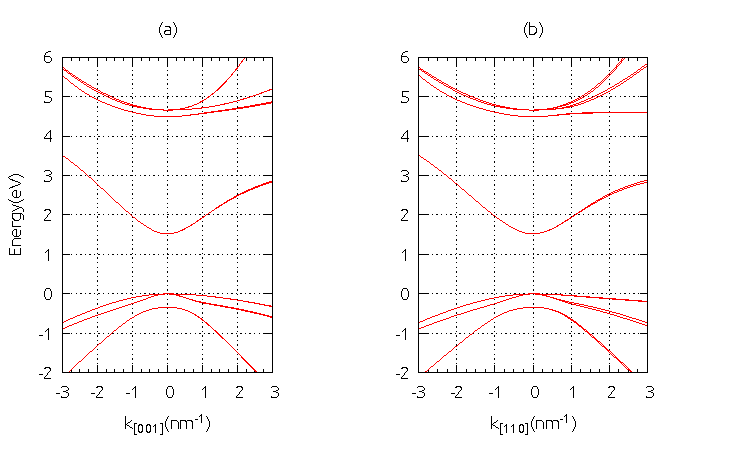
\includegraphics[width=0.70\textwidth]{./Figures/band-gaas.pdf}
%\rule{35em}{0.5pt}
\caption[computer kp 14-band GaAs]{Cấu trúc vùng năng lượng của chất bán dẫn GaAs bằng phương pháp kp $14\times14$ band, (a) $k\parallel[001]$ và (b) $k\parallel[110]$}
\label{fig:computer kp 14-band GaAs}
\end{figure}
Như chúng ta thấy ở ình 4.1 a thì độ tách mức năng lượng ở vùng hóa trị j=3/2 có độ tách không rõ ràng như ở hình b, còn đối với chất bán dẫn  GaInAs thì ngược lại ta thấy ở vùng hóa trị hình như ở hình a và b không có khác nhau cho lắm, còn ở vùng dẫn thì có sự khác nhau rõ ràng.
\begin{figure}[ht]
\centering
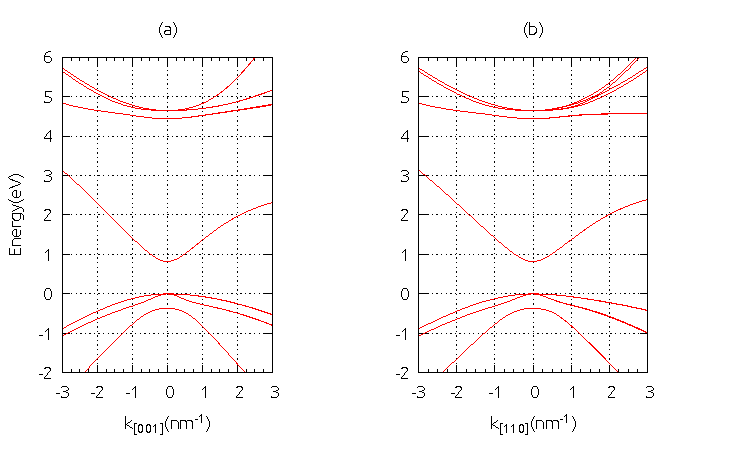
\includegraphics[width=0.70\textwidth]{./Figures/band-GaInAs.pdf}
%\rule{35em}{0.5pt}`
\caption[computer kp 14-band GaInAs]{Cấu trúc vùng năng lượng của chất bán dẫn GaInAs bằng phương pháp kp $14\times14$ band, (a) $k\parallel[001]$ và (b) $k\parallel[110]$}
\end{figure}

%\begin{figure}[ht]
%\centering
%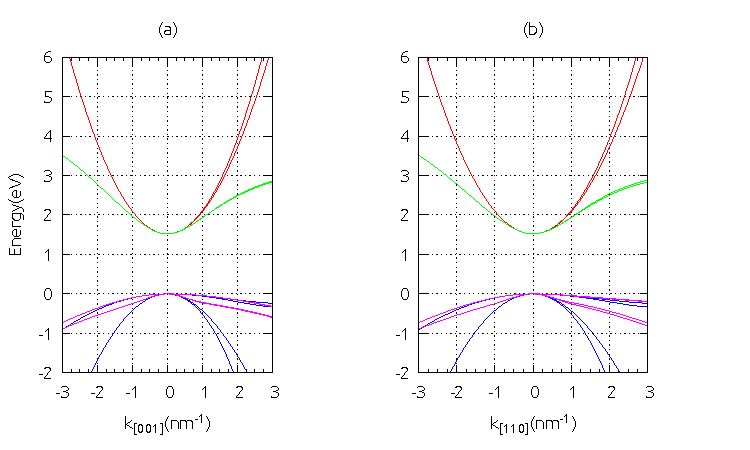
\includegraphics[width=0.70\textwidth]{./Figures/band14+lowdin.pdf}
%%\rule{35em}{0.5pt}
%\caption[computer kp 14-band and L$\ddot{o}$wdin GaAs]{Cấu trúc vùng năng lượng của chất bán dẫn GaAs bằng phương pháp kp $14\times14$ band màu xanh đậm và xanh dương(4-band đầu tiên của vùng hóa trị) và phương pháp L$\ddot{o}$wdin màu đỏ và tím(2 band đầu tiên của vùng dẫn), (a) $k\parallel[001]$ và (b) $k\parallel[110]$ }
%\end{figure}
\begin{figure}[ht]
\centering
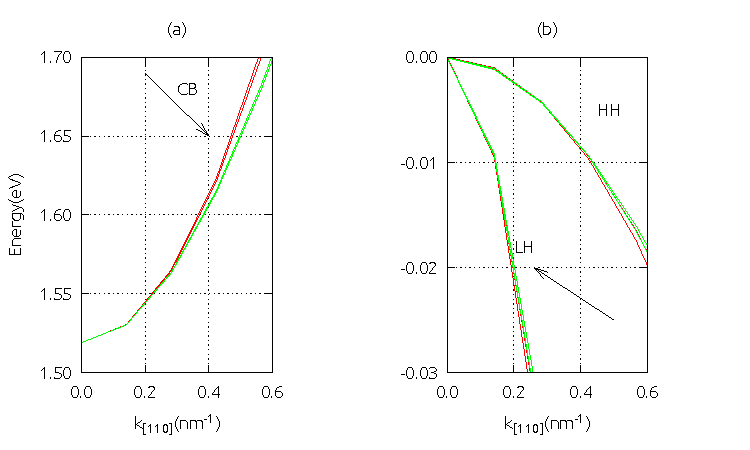
\includegraphics[width=0.70\textwidth]{./Figures/comparsion.pdf}
%\rule{35em}{0.5pt}
\caption[computer kp 14-band and L$\ddot{o}$wdin GaAs]{Cấu trúc vùng năng lượng của chất bán dẫn GaAs được tính bằng 2  phương pháp: kp $14\times14$ band màu xanh và L$\ddot{o}$wdin band  màu đỏ, (a) Độ phân tán của dãy dẫn và (b) Độ phân tán của dãy hóa trị}
\end{figure}
\begin{figure}[ht]
\raggedleft
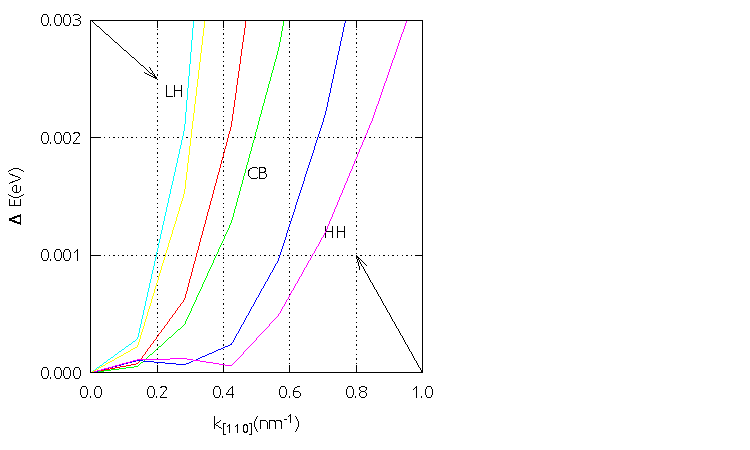
\includegraphics[width=0.70\textwidth]{./Figures/comparsion2.pdf}
%\rule{35em}{0.5pt}
\caption[so sánh phương pháp kp 14-band GaAs và L$\ddot{o}wdin$]{Độ tách suy biến của mức năng lượng spin up và spin down\\
 $\Delta E(k_{[110]})= \vert\Delta E(k_{[110]}.\uparrow) - \Delta E(k_{[110]}.\downarrow)\vert$}
\end{figure}